\chapter{Theory}

\section{Gamma-ray Spectroscopy}

In this section, the physics responsible for the features in gamma-ray spectra are described. Also described are factors that complicate gamma-ray spectroscopy, including changing background radiation fields and temperature effects on detector calibration.

% https://sites.fas.harvard.edu/~phys191r/Bench_Notes/B1/NAI_catalog.pdf page 20 has efficiency uncertainty information

\subsection{Energy Deposition Mechanisms}

When a photon interacts with a radiation detection medium (e.g. a NaI(Tl) crystal), it deposits some or all of its energy into the material. There are three main methods of interaction: the photoelectric effect, Compton scattering, and pair production. These effects are energy dependent, as seen in Figure \ref{fig:energy_dependence_interactions}.

If the photon's total energy is deposited in the detector, a count is recorded in the spectrum's photopeak. If the photon deposits only a part of its energy and escapes the detector, a count will be recorded somewhere below the full-energy photopeak.  The following sections describe intrinsic mechanisms that remove counts from the full-energy peak. % Absolute efficiency is also affected by shielding material and source-to-detector distance.


\subsubsection{Photoelectric Absorption}
% knoll pg 323

Photoelectric absorption is a process that can occur when a photon with energy, $E_{\gamma}$, greater than the binding energy of a bound electron, $E_{b}$, is absorbed by an atom. This absorption produces a photoelectron, which has the energy of the photon minus the binding energy of the electron
%
\begin{align} \label{eq:photoelectric_effect}
E_{e^{-}} &= E_{\gamma} - E_{b} \\
&= h\nu - E_{b} \\
\text{where } h &= \text{Planks Constant} \quad [J \cdot s] \nonumber \\
\nu &= \text{The Photon's Frequency} \quad \left[\frac{1}{\text{s}}\right] \nonumber \\
\end{align}
%
where $E_{\gamma}$ = $h\nu$ is the incident photon's energy. The photoelectron is typically absorbed by the material, resulting in full-energy deposition. This process also creates an electron vacancy in the original atom. This vacancy is filled by another electron in the material, releasing a characteristic x-ray or Auger electron. The characteristic x-ray can either be reabsorbed by the material or escape. Because of their low energies, Auger electrons are typically quickly reabsorbed.

\begin{figure}[H]
\centering
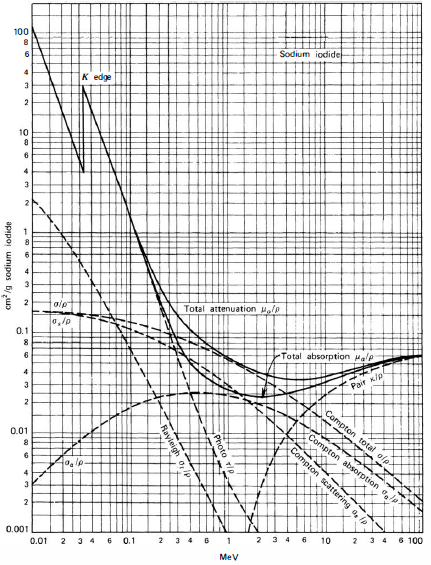
\includegraphics[width=0.75\linewidth]{images/energy_dependence_interactions}
\caption{Energy dependence for gamma-ray interactions in NaI(Tl). Reproduced from \cite{knoll}.}
\label{fig:energy_dependence_interactions}
\end{figure}

\subsubsection{Compton scattering}

Compton scattering is the interaction of a gamma-ray photon with an electron in absorbing material. This interaction is illustrated in Figure \ref{fig:compton_scatter}.


% This is the main energy deposition mechanism in the range of energies useful for gamma-ray spectroscopy.

\begin{figure}[H]
\centering
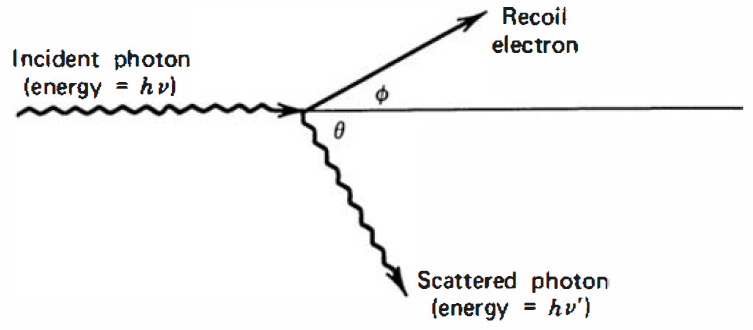
\includegraphics[width=0.7\linewidth]{images/compton_scatter}
\caption{Diagram of a Compton scattering event. Reproduced from \cite{knoll}.}
\label{fig:compton_scatter}
\end{figure}

The energy of a photon scattered off a free electron

\begin{equation} \label{eq:compton_scatter}
E_{\gamma}' = \frac{E_{\gamma}}{1 + \frac{E_{\gamma}}{m_{0} c^2} (1-cos\theta)}
\end{equation}

depends on the scattering angle, $\theta$, the incident photon's energy, E$_{\gamma}$, and the rest mass of the electron, m$_{o}$c$^{2}$. A photon scattering at an angle of 180$^{o}$ deposits its maximum amount of energy into a medium. Photons that escape after this energy deposition create the Compton edge observed at $\theta$ = 180$^{o}$, seen in the solid line in Figure \ref{fig:ideal_compton}. Photons that escape the detector after single or multiple Compton scatter events at angles less than 180$^{o}$ create the continuum of energies known as the Compton continuum. Accounting for the binding energy of electrons in a medium produces a Compton continuum more similar to the dotted line in Figure \ref{fig:ideal_compton}.

The Compton continuum of higher-energy photons will add to lower-energy photopeaks, adding noise to and changing the baseline of lower-energy photons' signals. The geometry between the source and detector changes the Compton continuum's shape, making the Compton continuum's signal difficult to incorporate into an identification algorithm. This signal can be incorporated into template matching or ANN based algorithms by including library or training set examples with various source-detector geometries.

\begin{figure}[H]
\centering
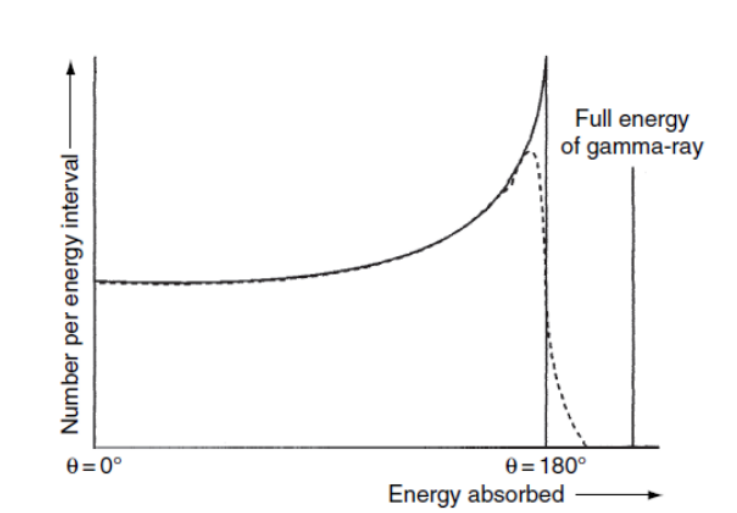
\includegraphics[width=0.75\linewidth]{images/ideal_compton}
\caption{Diagram of energy absorbed in an idealized Compton scattering event. The solid and dashed line represent idealized spectra with and without including electron binding energy. Reproduced from \cite{gilmore}.}
\label{fig:ideal_compton}
\end{figure}



\subsubsection{Pair Production}

When a photon with energy above 1022 keV (two times the rest mass energy of an electron) interacts with the Coulomb field of a nucleus, there is a probability that the photon will disappear and be replaced by an electron-positron pair. The positron will then annihilate with an electron in the medium, creating two 511 keV photons. This process is illustrated in Figure \ref{fig:pair_production}. If one or both of these annihilation photons escape the detector, they produce single or double escape peaks in a gamma-ray spectrum. As seen in Figure \ref{fig:pair_production_spectra}, single escape peaks occur at 511 keV below the full-energy peak and double escape peaks occur at 1022 keV below this peak. These 511 keV photons may also be measured by the detector, producing an annihilation radiation signal in the spectrum.

\begin{figure}[H]
\centering
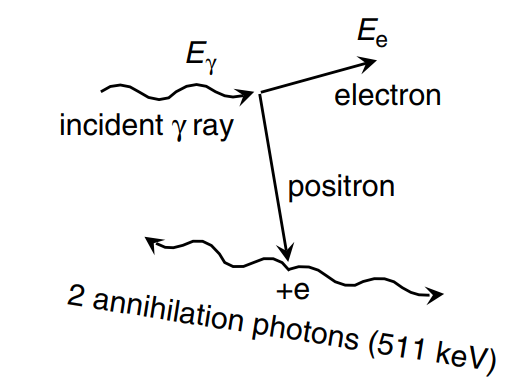
\includegraphics[width=0.6\linewidth]{images/pair_production}
\caption{Diagram of pair production. Reproduced from \cite{gilmore}.}
\label{fig:pair_production}
\end{figure}

\begin{figure}[H]
\centering
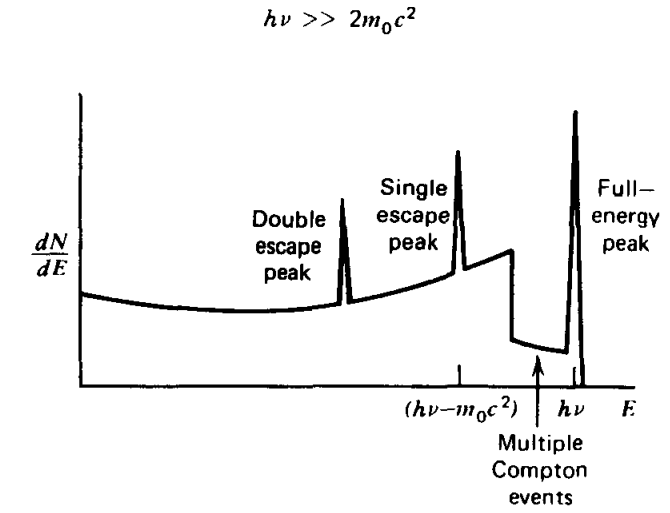
\includegraphics[width=0.6\linewidth]{images/pair_production_spectra}
\caption{Theoretical spectrum from pair production. Reproduced from \cite{knoll}.}
\label{fig:pair_production_spectra}
\end{figure}


\subsection{Energy Resolution} \label{subsection_energy_resolution}

The energy resolution of a radiation detector determines the photopeak's distribution, specifically the full width of its Gaussian peak at half of its maximum value (FWHM), at a location in a spectrum. The FWHM is measured either in units of energy or as a percent of the peak's energy. This broadening is mostly due to statistical fluctuations in the number of information carriers produced in the detection system. Other factors that increase the resolution in scintillation detectors include nonproportionality of light yield per energy absorbed, the variance in photoelectron collection in the photocathode, and the variance in electrons produced in the photomultiplier tube \cite{knoll}. Because semiconductor detectors more directly measure charge carriers, they do not suffer the resolution losses associated with transforming information carriers. The variance in information carriers produced for a given energy does not follow a Poisson process in semiconductor detectors. This effect is known as the Fano factor and it significantly decreases the resolution of semiconductor detectors below the theoretical Poisson limit \cite{knoll}. Because the resolution changes as function of energy, the resolution of a 662 keV photon from $^{137}$Cs is used as a standard for comparison. The energy resolution of three scintillator (NaI(Tl), LaBr, CeBr) and two semiconductor (CZT, HPGe) radiation detectors are compared in Table \ref{table:detector_resolutions}. Figure \ref{fig:Ba133_spectrum_different_detector_materials_Market_Survey_Report} compares a $^{133}$Ba spectrum as measured by scintillation and semiconductor detectors. 

% pg 345 knoll
\begin{table}[H]
\centering
\begin{tabular}{cc}
\hline
\textbf{Detector Type} & \begin{tabular}[c]{@{}c@{}}\textbf{Full Width at Half Maximum}\\ \textbf{(662 keV)}\end{tabular} \\ \hline
NaI(Tl) & 6 - 8 \% \\ % \hline
LaBr & 2 - 4 \% \\ % \hline
CeBr & 4 - 5 \% \\ % \hline
CZT & 1 - 2 \% \\ % \hline
HPGe & \textless 0.2 \% \\ \hline
\end{tabular}
\caption{Typical energy resolutions of common
gamma-ray detector types. Reproduced from \cite{RIIDMarketSurveyReport}.}
\label{table:detector_resolutions}
\end{table}


\begin{figure}[H]
\centering
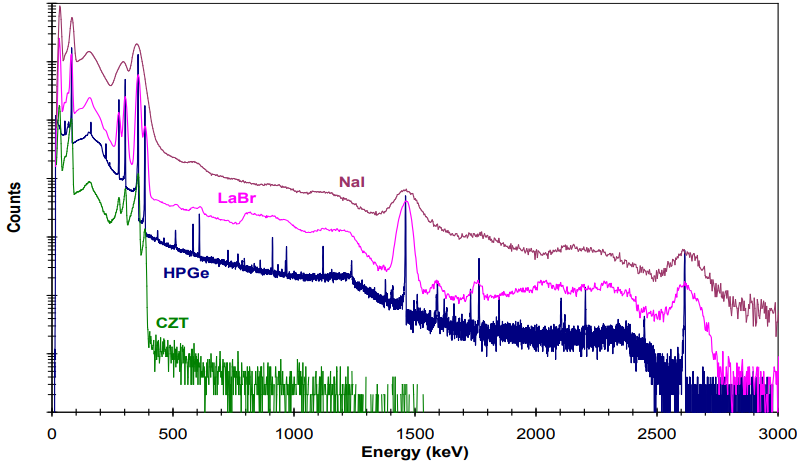
\includegraphics[trim=0 0 0 0, clip, width=1.0\linewidth]{images/Ba133_spectrum_different_detector_materials_Market_Survey_Report}
\caption{$^{133}$Ba spectrum measured using common detector materials. Reproduced from \cite{RIIDMarketSurveyReport}.}
\label{fig:Ba133_spectrum_different_detector_materials_Market_Survey_Report}
\end{figure}

Gamma-ray spectroscopy tasks in low resolution detectors, such as NaI(Tl), are complicated by overlapping photopeaks. Without well distinguished photopeaks, the signal from a source may be indistinguishable from noise or background. For example, in Figure \ref{fig:Ba133_spectrum_different_detector_materials_Market_Survey_Report} the two photopeaks around 600 keV are only clearly distinguishable in the high resolution HPGe detector. Wide photopeaks are also more likely to overlap with neighbors, potentially making them indistinguishable from each other, further complicating identification.


\subsection{Background Radiation}

% In contrast, it is extremely difficult to measure a trustworthy background spectrum in the field. Moving or reorienting the detector to obtain a source7free background measurement will frequently produce a measurement that will likely differ significantly, and sometimes even exceeding, the true background at the source position. It is not at all unusual for environmental background to vary significantly over distances of a few meters. As a result, we typically confine our analyses to the foreground spectrum, as generally reflected in this paper. https://e-reports-ext.llnl.gov/pdf/770028.pdf

A significant challenge to automated gamma-ray spectroscopy is the stochastic nature of the background radiation field. 
Spatial and temporal changes in background alter a gamma-ray spectrum's continuum and add a source of unwanted photopeaks. Background radiation comes from many sources including cosmic radiation and radioisotopes naturally distributed in soil and building materials. Isotopes in the soil primarily come from the uranium decay series, thorium  decay series, and $^{40}$K. The gamma-ray spectra from each of these sources are shown in Figure \ref{fig:background_components}. These background signals span the range of energies useful to gamma-ray spectroscopy, adding multiple sources of independent noise and complicating analysis.

\begin{figure}[H]
\centering
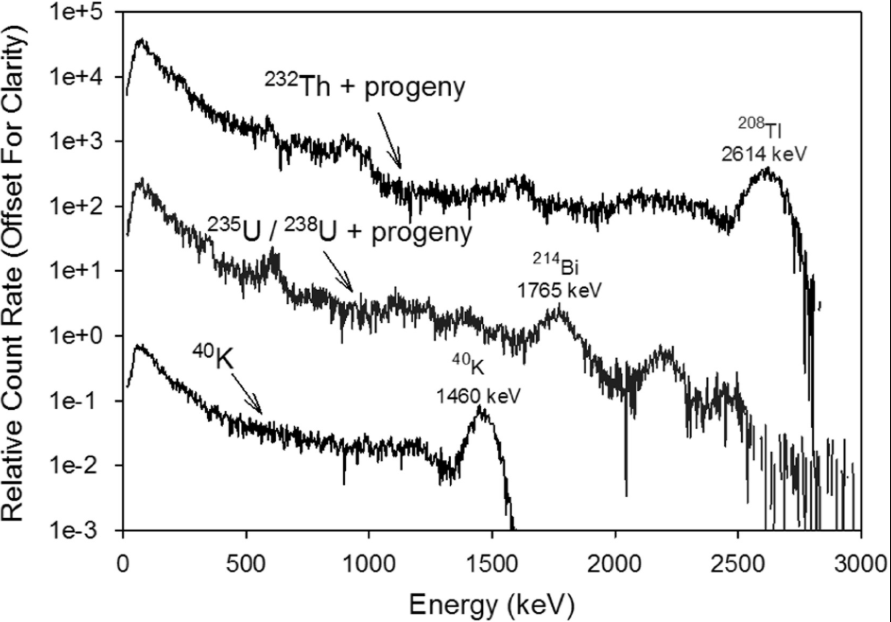
\includegraphics[width=0.8\linewidth]{images/background_components}
\caption{Monte Carlo simulations of background component spectra in NaI(Tl). Reproduced from \cite{KULISEK2015}.}
\label{fig:background_components}
\end{figure}

These radiation components can change both spatially and temporally. Because subsurface rocks vary in their elemental composition, background radiation isotope concentrations change geologically (Figures \ref{fig:USGS_u_conc}, \ref{fig:USGS_th_conc}, and \ref{fig:USGS_k_conc}). Local changes in soil composition and building materials also are significant enough to impact background. Because common building materials like concrete and granite contain radioactive elements, the proximity to these structures cause local variations in background. 

Background also changes over time, largely due to the decay products of $^{222}$Rn gas generated by uranium decay in soil \cite{knoll}. Rain can accordingly increase the level of background radiation by releasing trapped radon gas and other radioactive sources in the soil.

% Air Survey on Background Gradients https://www-sciencedirect-com.proxy2.library.illinois.edu/science/article/pii/S0265931X13002373

\begin{figure}[H]
\centering
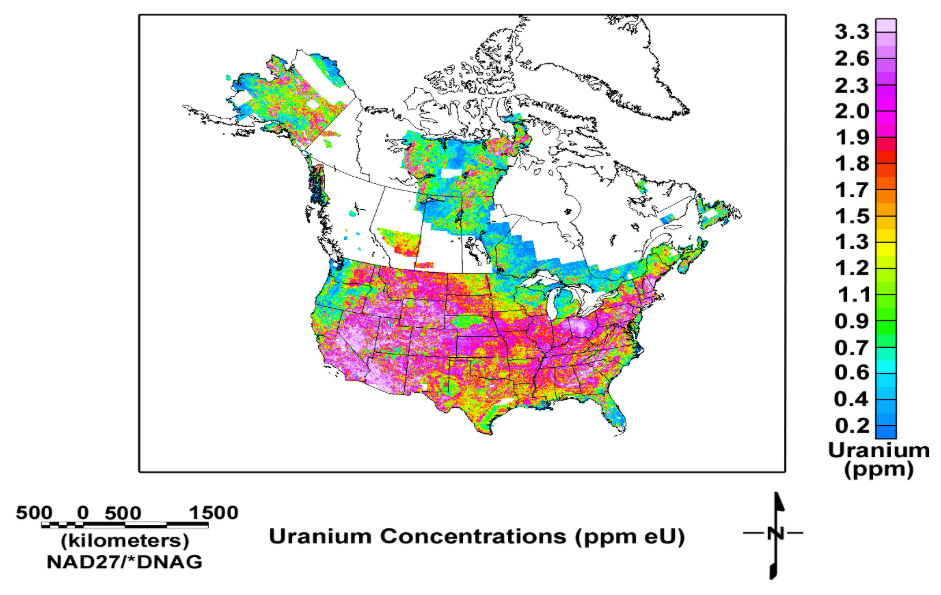
\includegraphics[trim=10 0 5 0, clip, width=1.0\linewidth]{images/USGS_u_conc}
\caption{Map of uranium concentrations in the United States. Reproduced from \cite{USGS}.}
\label{fig:USGS_u_conc}
\end{figure}

\begin{figure}[H]
\centering
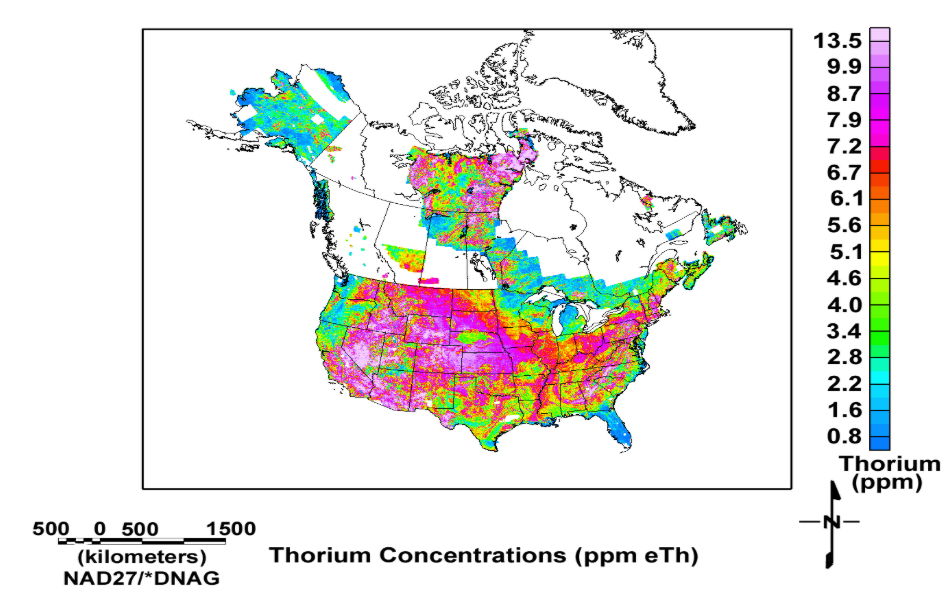
\includegraphics[trim=10 0 5 0, clip, width=1.0\linewidth]{images/USGS_th_conc}
\caption{Map of thorium concentrations in the United States. Reproduced from \cite{USGS}.}
\label{fig:USGS_th_conc}
\end{figure}

\begin{figure}[H]
\centering
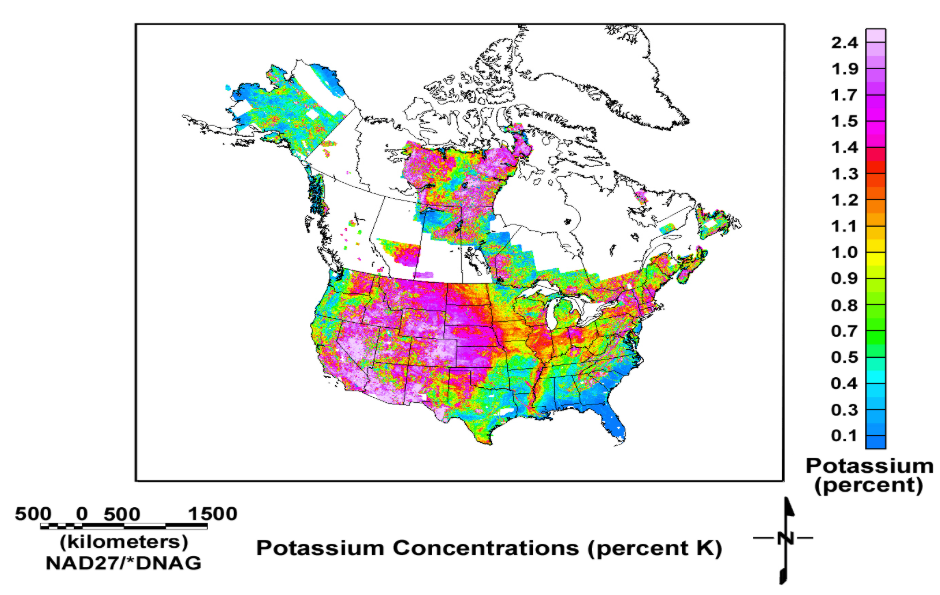
\includegraphics[trim=10 0 5 0, clip, width=1.0\linewidth]{images/USGS_k_conc}
\caption{Map of potassium concentrations in the United States. Reproduced from \cite{USGS}.}
\label{fig:USGS_k_conc}
\end{figure}


\subsection{Effect of Temperature on Calibration and Resolution}

% https://www.pnnl.gov/main/publications/external/technical_reports/pnnl-14735.pdf

The calibration of a NaI(Tl) detector can vary due to drifts in electronics, such as the dynode, and drifts in temperature of the crystal. Calibration drift has been identified as a key factor in the poor performance of RIIDs \cite{blackadar2003}. The distribution of the intensities of different NaI(Tl) scintillation light decay processes \cite{IANAKIEV2009432} and decay time constants of these processes \cite{MOSZYNSKI2006739} are sensitive to temperature. These factors lead to appreciable changes in relative photopeak position with temperature, shown in Figure \ref{fig:CASANOVAS2012588}, and detector resolution, shown in Figure \ref{fig:temp-dependence-resolution-moszynski}. 

While automated gain stabilization methods exist, many require a clear photopeak in the spectrum to calibrate from. This can be achieved with measurement times long enough to identify a background photopeak, attaching an external radioactive source to the detector, or by adding a reference light source. Measurement times long enough to identify a background photopeak may be infeasible for certain applications or the calibration step ignored altogether as a part of typical operation. Adding an external source of radiation adds additional noise to the spectrum. For these reasons, software-based, automated, gain stabilization techniques should be used to overcome this issue.

\begin{figure}[H]
\centering
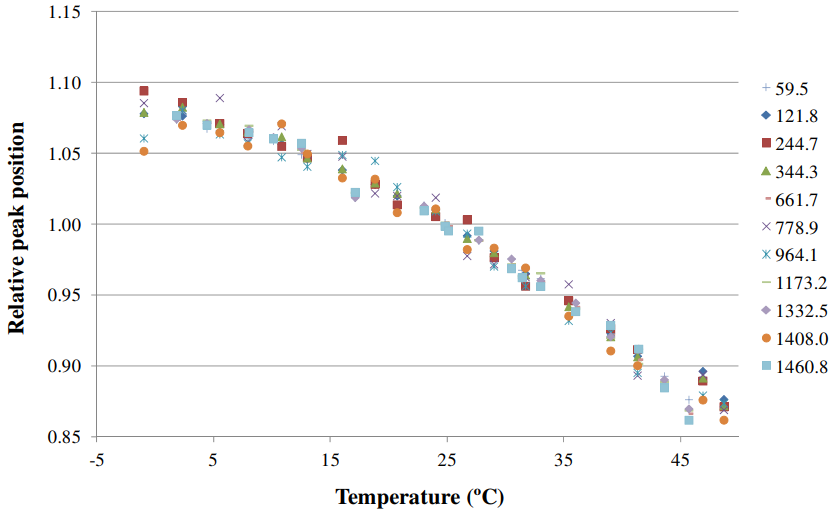
\includegraphics[width=0.95\linewidth]{images/temp_vs_relative_peak_position_CASANOVAS2012588}
\caption{Temperature vs relative photopeak position for an ORTEC Model 905-3 2x2 NaI(Tl) detector.  Reproduced from \cite{CASANOVAS2012588}.}
\label{fig:CASANOVAS2012588}
\end{figure}



\begin{figure}[H]
\centering
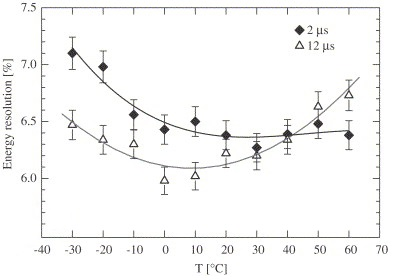
\includegraphics[width=0.95\linewidth]{images/temp-dependence-resolution-moszynski}
\caption{The energy resolution of 662 keV $\gamma$-rays measured with a 25mm x 30mm NaI(Tl) crystal using 2 $\mu$s and 12 $\mu$s peaking times. Reproduced from \cite{MOSZYNSKI2006739}.}
\label{fig:temp-dependence-resolution-moszynski}
\end{figure}

\section{Machine Learning}

In this section we describe the general theory behind how neural networks operate, how to train them, and how to optimize their architectures for a task. We also give an overview of the neural network architectures studied in this work and parameters that affect their training.

\subsection{General Neural Network Architecture}

An artificial neural network (ANN) is a mathematical model that attempts to map an arbitrary function from $\mathbb{R}{^M}$ to $\mathbb{R}{^N}$, where $M$ and $N$ are positive integers. An ANN accomplishes this by mimicking biological neurons. One example of an ANN architecture is shown in Figure \ref{fig:Network}. This ANN has N neurons in input layer A, J neurons in layer B, and K neurons in output layer C. Layer B is called a hidden layer because it is not directly observed in the input or output layers. Each neuron in adjacent layers is connected by a weight matrix, represented in Figure \ref{fig:Network} by arrows connecting neurons.


\begin{figure}[H]
\centering
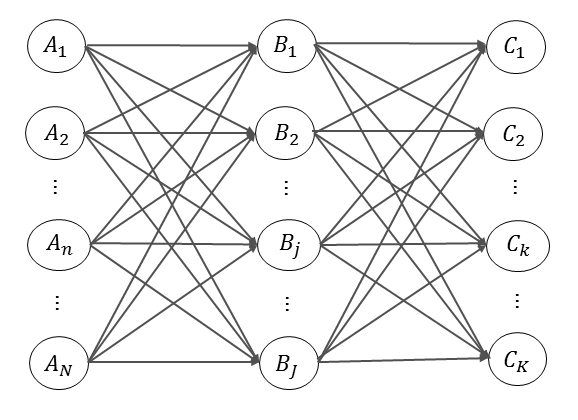
\includegraphics[width=0.75\linewidth]{images/Network}
\caption{Example ANN with input neurons $A_n$, hidden neurons $B_j$, and output neurons $C_k$ \cite{kamuda2017}.}
\label{fig:Network}
\end{figure}


Similar to a biological neuron, the ANN neuron receives input stimuli, performs an operation using it, and returns a signal. The structure and equation governing the operation of an individual neuron is shown in Figure \ref{fig:Node}. 

\begin{figure}[H]
	\centering
	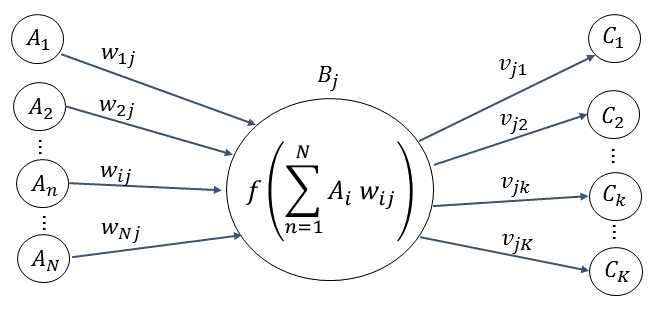
\includegraphics[width=0.75\linewidth]{images/Node_ABC_2}
	\caption{Summary of the operation of a single neuron \cite{kamuda2017}.}
	\label{fig:Node}
\end{figure}

As seen in Figure \ref{fig:Node}, each neuron operates by summing the products of the previous layer's values ($A{_1}$, $A{_2}$, ... $A{_N}$) and each individual weight ($w_{1j}$, $w_{2j}$, ... $w_{nj}$) connecting the neurons. This summation is analogous to the stimulus a biological neuron receives from its dendrites. A a non-linear activation function, $f$, operates on the total stimulus. The output signal is then passed to the next layer of the ANN where the process repeats. An ANN may be trained by finding a function, $f$, that solves
%
\begin{align} \label{eq:argminW_Error}
\underset{\mathbf{W}}{\text{argmin}} &{\text{ E}}(f(\mathbf{X} ; \mathbf{W} ) , \mathbf{T} ) \\
\text{where E} &= \text{error metric} \nonumber \\
\mathbf{W} &= \text{weight matrix} \nonumber \\
\mathbf{T} &= \text{target values} \nonumber \\
\mathbf{X} &= \text{input data.} \nonumber
\end{align}
%
Except in simple cases, Equation \ref{eq:argminW_Error} cannot be solved analytically. Numerical methods for solving this equation include gradient descent through the back-propagation of errors \cite{Rumelhart1986}, genetic learning algorithms \cite{Yao1999}, and Newton's method \cite{Fletcher2000}. In this work, we use a gradient descent implementation called Adam \cite{Kingma2015}. Adam is described in section \ref{section_training_algs}.

\subsection{Neural Network Training}

The most common ANN training method is applying gradient descent to the backpropagation of errors. The gradient we attempt to minimize is the derivative of an error metric with respect to the network's weights and biases. These gradients show how the networks weights and biases need to change,
%
\begin{align}
\Delta w_{j} &= - \eta \frac{dE(D)}{dw_j} \label{eq:update1} \\
\Delta b_{j} &= - \eta \frac{dE(D)}{db_j} \label{eq:update2} \\
\text{where E} &= \text{error metric} \nonumber \\
\eta &= \text{learning rate,} \nonumber
\end{align}
% The learning rate determines the update step's size.
to reduce the error metric for some training data,
%
\begin{align} \label{eq:train_data_D}
D&={(\boldsymbol{x}_1,t_1), ... , (\boldsymbol{x}_n,t_n), ... , (\boldsymbol{x}_N,t_N)}, \\
\text{where } \boldsymbol{x}_{n} &= n^{th} \text{ training example} \nonumber \\
t_n &= n^{th} \text{ training target.} \nonumber
\end{align}
%
The learning rate and its affect on training are discussed further in section \ref{LearningRateSubsection}. Using these equations, the gradients can be repeatedly measured to iteratively update the weights. Updating the network with the entire dataset only once is referred to as one training epoch. Due to computational constraints involving memory, it is often infeasible to calculate the update rules in Equations \ref{eq:update1} and \ref{eq:update2} for the entire training dataset. A common technique used to train on large datasets is to iteratively update weights using disjoint subsets of the training data, called minibatches.

Training occurs until an early stopping condition is met. Early stopping works by first removing a portion of the training data and defining it as validation data. The ANN is trained using the new training data while we monitor an error metric for the training and validation datasets. Early stopping conditions include ending training when a threshold on an error metric measured in the validation dataset is reached or when the error metric has not improved (either by some factor or absolutely) in a fixed number of epochs, called the early stopping patience. 

Early stopping is needed to end training when the model begins to overfit or learning plateaus. Overfitting occurs when the validation dataset's error increases and the training dataset's error decreases, illustrated in Figure \ref{fig:training_testing_error}. This indicates that the model is memorizing the training data and not generalizing to examples not seen during training. Generalization is a term used to describe a model's performance on unseen data. Learning can also plateau when the ANN's weight updates are not large enough to escape a minimum in the error metric measured on the training dataset.

\begin{figure}[H]
	\centering
	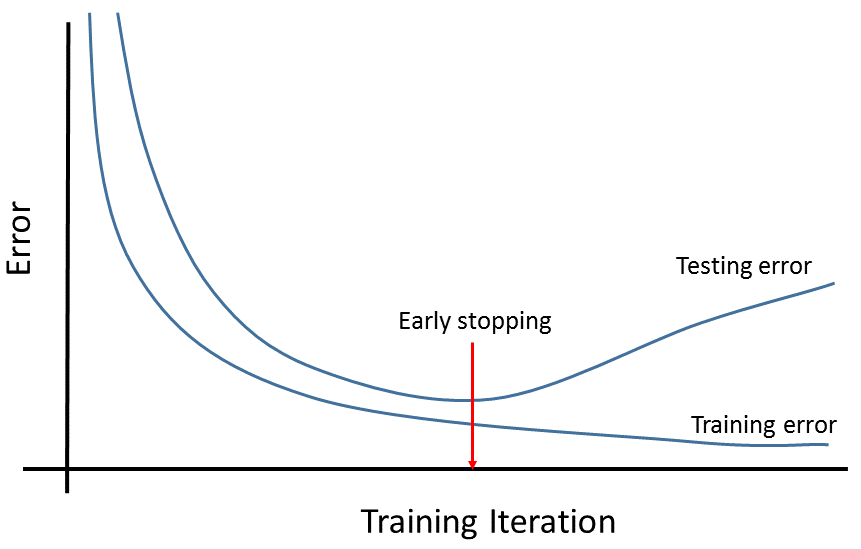
\includegraphics[trim=0 190 390 0,clip,width=0.7\linewidth]{images/training_testing_error_v2}
	\caption{Example training and validation error curves.}
	\label{fig:training_testing_error}
\end{figure}

A common technique for choosing training and validation data is k-folds cross validation. Figure \ref{fig:kfolds} illustrates 5-folds cross validation. In this process, $\frac{1}{k}$ of all available data is split into a validation dataset and the rest is defined as the training dataset. The model is then trained using the training data and the validation dataset's error is recorded. The process of splitting the dataset is repeated k times. The average error metric of each trained model on the validation dataset is used to estimate the generalization capabilities of the overall model. In this work, we use 5-folds cross validation to 


\begin{figure}[H]
	\centering
	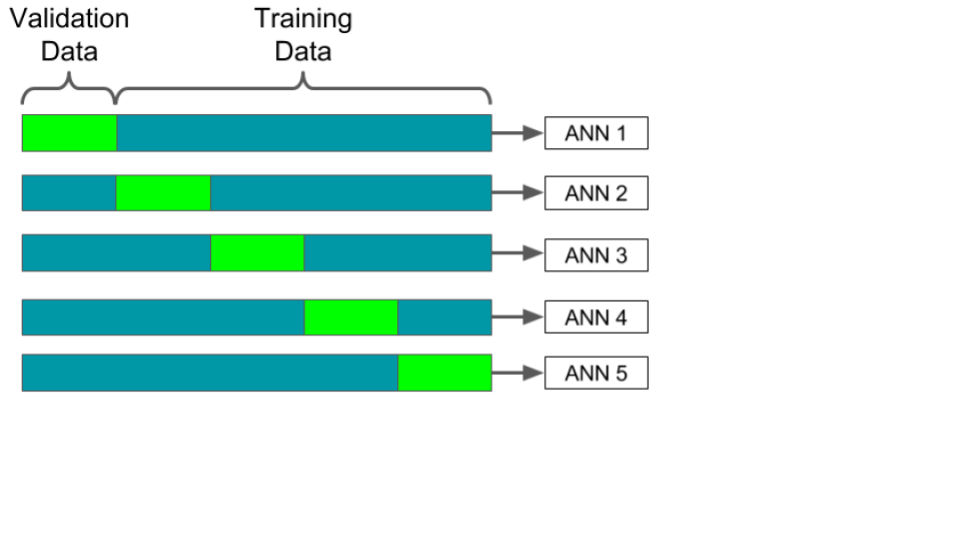
\includegraphics[trim=0 140 310 0,clip,width=0.7\linewidth]{images/kfolds}
	\caption{An example of k-folds cross validation.}
	\label{fig:kfolds}
\end{figure}

\subsection{Simple Neural Network Example}

An example of a simple one-layer ANN is shown in Figure \ref{fig:one_layer_net}. This ANN is a function that takes two real-valued inputs ($x_1$ and $x_2$) and performs the operation shown in Figure \ref{fig:Node}. The weights in the hidden layer connecting the $i^{th}$ input neuron to the $j^{th}$ output neuron are represented by $w_{ij}$. An extra node, called the bias, is added to make the layer affine. Without the bias, the layer would be linear, meaning an input vector of zeros could only be mapped to another vector of zeros. The bias allows for more expressive mappings, adding to the representational power of the model. The bias activation is set to a constant value of 1, allowing the bias to be trained by changing the weights connecting the bias to the next layer. Using the hyperbolic tangent function, the network outputs for each class $y_1$, $y_2$, and $y_3$ range [-1, 1]. Using this function, if an input results in the $y_{j}^{th}$ output neuron rising above zero, that input can be classified as part of the ${j}^{th}$ class (or as not a part of the ${j}^{th}$ class if the output is below zero). Other functions that map outputs values to arbitrary bounds (e.g. other sigmoid functions or an unbounded linear function) can be used. The equation for the output corresponding to the $j^{th}$ class is 
%
\begin{align} \label{eq:single_layer_eq_sum}
y_j &= \tanh(\sum_i x_i w_{ij} + b_j), \\
\text{where } y_j &= j^{th} \text{ output activation} \nonumber \\
x_i &= i^{th} \text{ input from the previous layer} \nonumber \\
b_j &= \text{weight connecting the } j^{th} \text{ output to the bias neuron.} \nonumber
\end{align}
%
\begin{figure}[H]
	\centering
	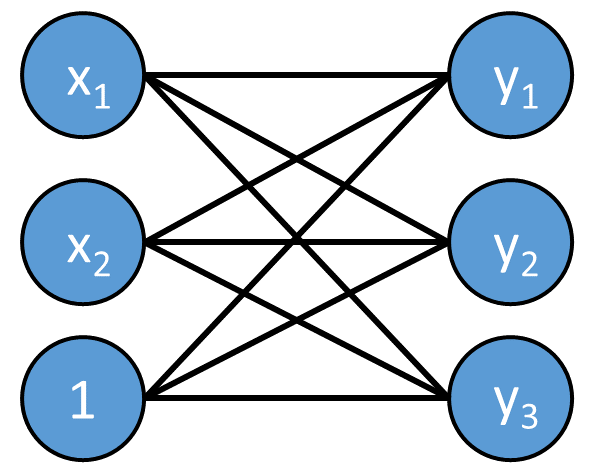
\includegraphics[width=0.45\linewidth]{images/One_layer_net_v31}
	\caption{Example of a single-layer neural network with two inputs ($x_{1}$ and $x_{2}$), three classes ($y_{1}$, $y_{2}$, $y_{3}$), and a bias neuron set to one.}
	\label{fig:one_layer_net}
\end{figure}
%
The geometry of the above network's operation is illustrated for an example dataset in Figure \ref{fig:training_set_one_layer}. This dataset is composed of three classes: red, green, and blue. The axes that define this dataset are the inputs to the single layer network in Figure \ref{fig:one_layer_net}, ($x_1$,$x_2$). If $\mathbf{W}$ is defined to be a vector with elements ($w_{11}$, $w_{21}$), a line can be defined perpendicular to $\mathbf{W}$ and shifted by $\frac{b_1}{||\mathbf{W}||}$ from the origin in the direction of $\mathbf{W}$. Given appropriate values for $w_{11}$, $w_{21}$, and $b_1$, a line that separates the blue class from the non-blue class can be created. Any point on the -$\mathbf{W}$ side of the line will have $y_1 < 0$, allowing for classification. Similarly, a separating line for the red class using $w_{12}$, $w_{22}$, and $b_2$ and a separating line for the green class using $w_{13}$, $w_{23}$, and $b_3$ can be constructed. 
\begin{figure}[H]
	\centering
	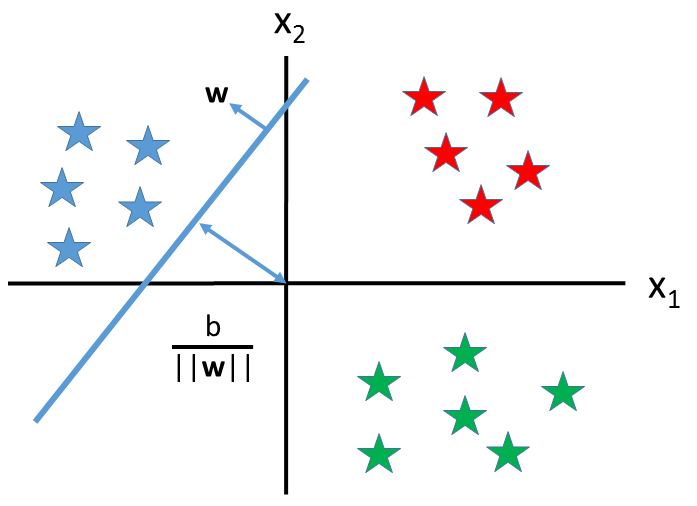
\includegraphics[width=0.65\linewidth]{images/training_set_for_single_layer_hyperplane_v2}
	\caption{A dataset describing a three class function. Each class is represented by a different color.}
	\label{fig:training_set_one_layer}
\end{figure}

The classes in this example dataset are linearly separable, meaning lines can be drawn completely separating each class. If the classes were not linearly separable, additional hidden layers would be necessary to compute the function. It has been shown that additional hidden layers allow the creation of arbitrary decision boundaries \cite{Hornik1991}. 


Backpropagation uses the chain rule to find these derivatives for some training data and target. Applying backpropogation in a single-layer ANN requires finding an expression for the derivative of an error function with respect to the networks weights \cite{Nielsen2015}. For example, to apply backpropogation when using the mean squared error function, E$_{MSE}$, on the network described in Equation \ref{eq:single_layer_eq_sum}, we apply the chain rule to find an expression for
%
\begin{align} \label{eq:dMSE}
\frac{dE_{MSE}}{dw_j} &= \frac{dE_{MSE}}{dy_i} \frac{dy_i}{dw_j}.
\end{align}
%
Equation \ref{eq:dMSE} can be solved by first evaluating $\frac{dE_{MSE}}{dy_i}$,
%
\begin{align} \label{dE_{MSE}/dy_i}
\frac{dE_{MSE}}{dy_i}  &= \frac{d}{dy_i} \frac{1}{N} \sum_{i=1}^N(t_i - y_i)^2 \\
&= \frac{1}{N} \sum_{i=1}^N  \frac{d}{dy_i} (t_i - y_i)^2 \nonumber \\
&=  -\frac{2}{N} \sum_{i=1}^N  (t_i - y_i). \nonumber
\end{align}
%
Evaluating $\frac{dy_i}{dw_j}$,
%
\begin{align} \label{dy_i/dw_i}
\frac{dy_i}{dw_j}  &= \frac{d}{dw_j} \tanh( \boldsymbol{w}' \boldsymbol{x}_i + b) \\
&= \tanh'( \boldsymbol{w}' \boldsymbol{x}_i + b) \frac{d}{dw_j}( \boldsymbol{w}' \boldsymbol{x}_i + b) \nonumber \\
&= \tanh'( \boldsymbol{w}' \boldsymbol{x}_i + b)  x_{ij}. \nonumber
\end{align}
%
\noindent where $x_{ij}$ is the $j^{th}$ index of the $i^{th}$ training vector.
%
The update rule for the bias is found using
%
\begin{equation} \label{eq:dE_MSE/db_j}
\frac{dE_{MSE}}{db_j} = \frac{dE_{MSE}}{dy_i} \frac{dy_i}{db_j}.
\end{equation}
%
The expression for $\frac{dE_{MSE}}{dy_i}$ is known from Equation \ref{dy_i/dw_i}. Evaluating the other derivative in \ref{eq:dE_MSE/db_j} we find
%
\begin{align}
\frac{dy_i}{db_j} &= \frac{d}{db_j} \tanh(\boldsymbol{w}'\boldsymbol{x}_i + b) \\
 &= \tanh'( \boldsymbol{w}' \boldsymbol{x}_i + b). \nonumber
\end{align}
Finally, the gradient of the error metric can be computed for a single weight, 
%
\begin{equation} \label{eq:dE_{MSE}/dw_j_final}
\frac{dE_{MSE}}{dw_j} =  -\frac{2}{N} \sum_{i=1}^N  (t_i - y_i) \tanh'( \boldsymbol{w}' \boldsymbol{x}_i + b)  x_{ij},
\end{equation}
%
and a single bias,
%
\begin{equation} \label{eq:dE_{MSE}/db_j_final}
\frac{dE_{MSE}}{db_j} =  -\frac{2}{N} \sum_{i=1}^N  (t_i - y_i) \tanh'( \boldsymbol{w}' \boldsymbol{x}_i + b).
\end{equation}

Gradient descent can be applied to an ANN with multiple layers. The input to the the $l^{th}$ layer given some training example $\boldsymbol{x}$ in an L-layer network is 
\begin{equation}
\boldsymbol{z}^{x,l} = \boldsymbol{w}^{l}  \boldsymbol{a}^{x,l-1} + \boldsymbol{b}^{l}
\end{equation}
%
where the activation from the $(l-1)^{th}$ layer is
%
\begin{equation}
\boldsymbol{a}^{x,l-1} = f^{l-1}(\boldsymbol{z}^{x,l-1})
\end{equation}
\begin{align*}
  \text{and where } \boldsymbol{w}^{l} &= \text{weight matrix of layer l,} \\
  \boldsymbol{b}^{l} &= \text{bias vector of layer l,} \\
  f^{l-1} &= \text{non-linear activation function used in layer (l-1).}
\end{align*}
%
Defining the output error as 
%
\begin{equation}
\delta^{x,L} = \frac{\partial C}{\partial a^{x,L}} \odot \frac{\partial f^{l-1}(\boldsymbol{z}^{x,l-1}) }{\partial \boldsymbol{z}^{x,l-1}}, 
\end{equation}
%
where $\odot$ is the element-wise product, the output error can backpropagate to previous layers. For each $l=L-1,L-2,...,2$ an error can be defined by
%
\begin{equation}
\delta^{x,l} = ((\boldsymbol{w}^{l+1})^T \delta^{l+1}) \odot \frac{\partial f^{l}(\boldsymbol{z}^{x,l}) }{\partial \boldsymbol{z}^{x,l}}.
\end{equation}
%
The gradient of the cost function as a function of each individual weight and bias can now be defined as 
%
\begin{equation} \label{eq:CrossEntropy1}
\frac{\partial E}{\partial w_{jk}} = a^{l-1}_k \delta^l_j
\end{equation}
%
and 
%
\begin{equation} \label{eq:CrossEntropy2}
\frac{\partial E}{\partial b_j} = \delta^l_j.
\end{equation}
%
Using Equations \ref{eq:CrossEntropy1} and \ref{eq:CrossEntropy2}, the weights can be updated for a single backpropogation iteration. 


\subsection{Hyperparameters}

In addition to the weights connecting neurons, \textit{hyperparameters} can modify ANN behavior. Hyperparameters determine both the network's structure (number of layers, number of nodes in each layer, activation function for each layer) and how the model learns (learning rate, momentum, loss function). The following section discusses various hyperparameters and their effects on ANN learning.

The hyperparameters and their ranges used to optimize dense and convolutional models in this dissertation are shown in Tables \ref{table:hyperparameter_dataset_parameters_DNN} and \ref{table:hyperparameter_dataset_parameters_CNN}, respectively. Methods for hyperparameter  optimization are discussed in Section \ref{section_hp_opt}. The hyperparameter ranges explored in this dissertation are base on our published work \cite{kamuda2017, kamuda2018, kamudaThesis2017}.

\subsubsection{Learning Rate} \label{LearningRateSubsection}

The learning rate , $\eta$, affects the magnitude of each weight update. If $\eta$ is too small, the network will learn slowly and training will be inefficient. If $\eta$ is too large, the network will fail to learn, either by converging to a non-extremum or by diverging. An example of a small and large learning rate are shown in Figure \ref{fig:Learning_rate_comparison} 

\begin{figure}[H]
	\centering
	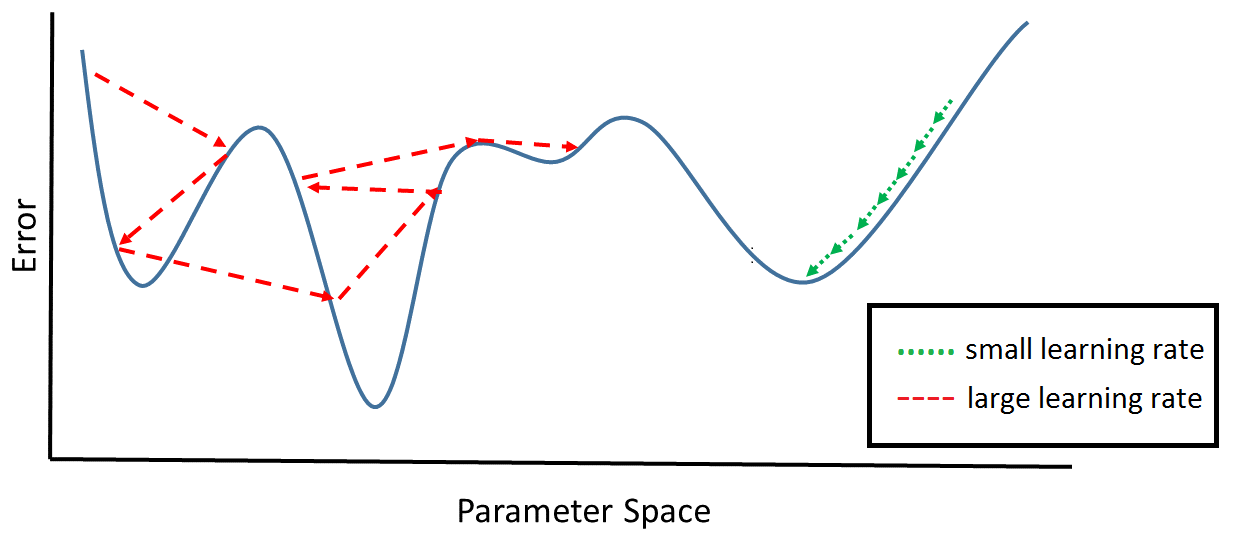
\includegraphics[width=0.8\linewidth]{images/Learning_rate_comparison_v2}
	\caption{Example training paths for a large learning rate and a small learning rate.}
	\label{fig:Learning_rate_comparison}
\end{figure}


There are many methods to modify $\eta$ to encourage more efficient learning. One method to increase the speed of learning is to start with a large $\eta$ and decrease $\eta$ as a function of iteration number. Ideally, this method would lead to quick initial learning when far from an optima and slower learning near an optima to more finely explore it. The difficulty with this method is the requirement for a function that slows the learning rate efficiently for a given problem.

% \subsubsection{Learning Momentum}

% Another method to speed up learning is to add a momentum hyperparameter, $\mu$, to the weight update algorithm \cite{Yu1997}, 
%
% \begin{equation} \label{eq:update_momentum}
% \Delta w_{ij}(n) = - \eta \frac{dE_{MSE}}{dw_j} +\mu \Delta w_{ij}(n-1).
% \end{equation}
%
% Similar to the goal of slowing learning over time described above, the momentum term attempts to slow learning near optima. The momentum will be large when % the weights are updated at large steps, far from an optima, but will decrease near an optimum, allowing slower learning near an optimum. 

\subsubsection{Training Algorithms} \label{section_training_algs}

There are many ANN training algorithms that employ various learning rate schedules and momentum functions. These algorithms include but are not limited to: Nesterov's accelerated gradient \cite{nesterov1983}, simulated annealing \cite{Kirkpatrick1983}, ADADELTA (An Adaptive Learning Rate Method) \cite{ADADELTA}, and Adam (Adaptive Moment Estimation) \cite{Kingma2015}. 

% Adam incorporates of parts of RMSprop and AdaGrad.
In this thesis, the Adam optimizer as implemented by TensorFlow \cite{tensorflow2015-whitepaper} was chosen as the training algorithm. The Adam optimizer is widely used due to training speedups and performance improvements on popular benchmark datasets like MNIST \cite{lecun98}, IMDB movie reviews \cite{Maas2011}, and CIFAR-10 \cite{Krizhevsky2009}. Another benefit of Adam is the introduction of effectively only one hyperparameter, the learning rate.

The ADAM optimizer update rule is described below. For the following, $g_t$ is the gradient of the error function with respect to the network parameters at iteration $t$, 
\begin{equation} \label{eq:adam1}
m_t = \beta_1 m_{t-1} + (1 - \beta_1) g_t,
\end{equation}
is the estimate of the mean of the gradient at iteration $t$ and
\begin{equation} \label{eq:adam2}
v_t = \beta_2 v_{t-1} + (1 - \beta_2) g_t^2
\end{equation}
is the estimate of the variance of the gradient at iteration $t$. For the following, the variables $\beta_1$ and $\beta_2$ are parameters called decay rates, $\epsilon$ is included for numerical stability, and $\theta_t$ represents the network parameters at iteration $t$. As described by Kingma and Lei Ba, the default values for $\beta_1$, $\beta_2$, and $\epsilon$ are 0.9, 0.999, and $10^{-8}$ respectively \cite{Kingma2015}. These values were seen to work well for a variety of problems. While these hyperparameters can also be tuned, it has been shown that the default values work well for a variety of network architectures and datasets \cite{Kingma2015}. The bias-corrected first moment estimate is given by
\begin{equation} \label{eq:adam3}
\hat{m}_t = \dfrac{m_t}{1 - \beta^t_1}
\end{equation}
and the bias-corrected second moment estimate is given by 
\begin{equation} \label{eq:adam4}
\hat{v}_t = \dfrac{v_t}{1 - \beta^t_2}.
\end{equation}
Finally, the weight update equation is computed as
\begin{equation} \label{eq:adam5}
\theta_{t+1} = \theta_{t} - \dfrac{\eta}{\sqrt{\hat{v}_t} + \epsilon} \hat{m}_t.
\end{equation}


%Due to the number of free parameters in a ANN (each hidden layer weight is a free parameter), these models have a tendency to overfit data. The three methods used to prevent overfitting in this thesis are $L_2$ regularization, neuron dropout, and data augmentation. These techniques greatly improve the performance of the presented ANN. 

% Is this neccesary? Just mentioning it is enough I think.

%Another method is to randomly perturbing the weights during training using a simulated annealing technique \cite{Kirkpatrick1983}. Simulated annealing mimics how crystal lattices bond together in cooling metal to achieve a low energy state. As metal cools, its crystal lattice will orient itself to lower its total bond energy, but occasionally due to statistical heating sections will jump to a higher energy level. This encourages a global low energy state, as many local low energy state regions are discouraged. This process can be mimicked in a learning algorithm by randomly perturbing the weights during learning. As learning continues the network 'cools' and the frequency of weight perturbation decreases. It can be shown that given a long enough annealing schedule, the global optimum solution for a problem is guaranteed to be found \cite{Granville1994}.

\subsubsection{Cost Functions and Performance Metrics}

The choice of cost function to train against depends on the targets the network is attempting to learn. One of the simplest error functions is the binary accuracy for classification, 
%
\begin{align} \label{eq:Binary_accuracy}
E_{Binary} &= {\frac{1} N} \sum_{n=1}^N \mathds{1}_[\hat{y}_n \neq y_n ], \\
\text{where } N &= \text{ number of output neurons} \nonumber \\
y_n &= n^{th} \text{ output neuron's ground truth} \nonumber \\
\hat{y}_n &= n^{th} \text{ output neuron's value} \nonumber \\
\mathds{1}_A &= \text{indicator function} \nonumber \\
&= \nonumber
\begin{cases}
1  & \quad \text{if } A \text{ is True}\\
0  & \quad \text{if } A \text{ is False.}
\end{cases} \nonumber
\end{align}
% where N is the total number of output neurons, $y_n$ is the ground truth of the n$^{th}$ output, and $\hat{y}_n$ is the ANN output of the n$^{th}$ output neuron. 
While this is a simple function, it cannot be used to train a gradient descent algorithm because it is discontinuous (there is no incremental indication that a model is improving).

A simple differentiable cost function is the mean squared error function,
%
\begin{equation} \label{eq:MSE_error}
E_{MSE} = {\frac{1} N} \sum_{n=1}^N (\hat{y}_n - y_n)^2.
\end{equation}
%
Because this function is differentiable, it can be used to train a gradient descent algorithm. The MSE function is appropriate when targets are any real number, as in a regression problem. The MSE cost function is used in the uranium enrichment regression problem in Chapter \ref{uranium-enrichment}. This cost function is also used when training autoencoders. An autoencoder is an ANN that attempts to reconstruct an input signal. Autoencoders are described in more detail in Section \ref{Autoencoders}. The autoencoders used in this work employ the MSE cost function.

For multi-class classification problems, the mean cross entropy,
%
\begin{equation} \label{eq:CrossEntropy}
E_{MCE} = -{\frac{1} N} \sum_{n=1}^N y_n \log(\hat{y}_n), 
\end{equation}
%
can be used as a cost function. Cross entropy measures the similarity between two probability distributions. By using cross entropy with the softmax output function,
%
\begin{equation} \label{eq:softmax}
softmax(z_j) = \frac{\exp(z_j)} {\sum_{k=1}^{K} \exp(z_k)},
\end{equation}
%
we can calculate the posterior probability of each class \cite{Bridle1990}. The cross entropy cost function and softmax output function are used in the source interdiction classification problem analyzed in Chapters \ref{ChapterMachineLearningModelsExplored} and \ref{UrbanSourceIdentificationResultsandDiscussion}.


% The softmax function normalizes an input vector into a probability distribution. Softmax is used as the output function for classification problems with multiple independent classes.

\subsubsection{Weight Regularization}

Weight regularization is a hyperparameter that penalizes the ANN when the magnitude of the weights increases. Because the magnitude of the weights is tied to the complexity of the model, adding weight regularization attempts to limit complexity and the probability of overfitting.

A common method of incorporating weight regularization is by adding an $L_n$ regularization term to the error function, 
%
\begin{equation} \label{eq:L2_Reg}
\tilde{E} = E + \sum_i \lambda w_i^n.
\end{equation}
%
Common values for $n$ are 1 and 2. Adding weight regularization allows the magnitude of the weights to increase only when there is a comparable reduction in the unmodified error function.

In Equation \ref{eq:L2_Reg}, $w_i$ is the weight between each neuron in the ANN and $\lambda$ is the regularization strength hyperparameter. A larger $\lambda$ will force the ANN to prefer smaller weights connecting the neurons. If the parameter $\lambda$ is too small, the unbounded model complexity may fit only the training data. If the parameter $\lambda$ is too large, the ANN will only minimize the $L_n$ error, failing to learn.

In this dissertation, $L_2$ weight regularization is added to the densely connected portions of the classification networks. In our published work, we employed $L_2$ weight regularization as a hyperparameter to regularize our models.

\subsubsection{Neuron Dropout}

Another method to reduce model complexity is by adding a \textit{neuron dropout rate} hyperparameter. Neuron dropout is the process of temporarily removing a random set of neuron from the ANN architecture during each training iteration \cite{Srivastava2014}.

Almost always, taking the average output of more than one separately trained ANN improves the performance of the ANN \cite{Srivastava2014}. By applying dropout at each neuron with the same probability throughout training, the ANN's architecture changes every iteration. This makes neuron dropout a cost efficient way to effectively average many different ANN architectures, improving performance. 

% Without dropout, local codependency between neurons that could lead to the ANN becoming stuck in a local minimum in the error function. By randomly removing neurons from an ANN during training, - and thus overtraining - is discouraged. The frequency with which neurons are removed is called the neuron dropout rate.

In this dissertation, neuron dropout is added to the densely connected portions of the classification networks. In our published work, we employed neuron dropout as a hyperparameter to regularize our models.


\subsubsection{Data Augmentation}

Machine learning algorithms perform better with more data. To increase the amount of data available, before each training iteration the input data can be randomly modified using physically realistic transformations. This process is called online \textit{data augmentation}. Data augmentation can be performed either online or offline. Online data augmentation refers to applying the augmentation during each training batch, ensuring the network never sees the same data twice. If augmenting the data is computationally expensive, this method can slow training - potentially prohibitively. Offline data augmentation is used to expand the dataset before training. This can be used to reduce computational costs during training at the expense of storing the additional data.

For example, a training dataset of images can be rotated, flipped, blurred, or brightened during training. An example of horizontal flip and a blur augmentation are seen in Figure \ref{fig:cat}. Both the augmentation method and parameters of the method (e.g. degrees rotated, Gaussian blur variance) are hyperparameters.



\begin{figure}[H]
	\centering
	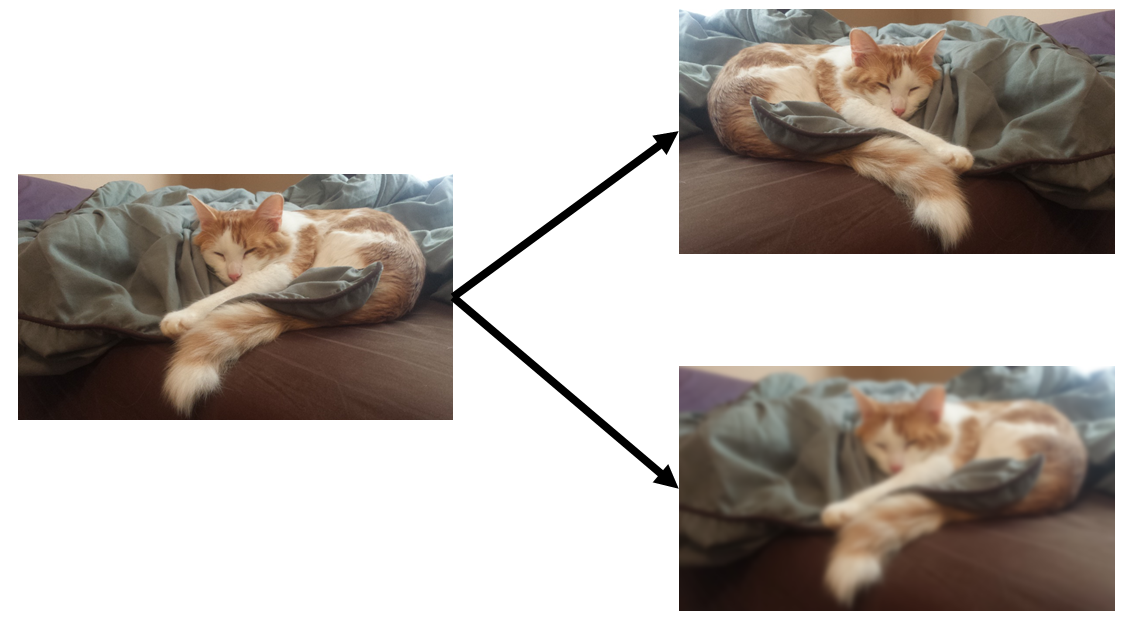
\includegraphics[width=0.9\linewidth]{images/cat}
	\caption{Two examples of data augmentation using an image of a cat. The image to the left is the original. The top right image is augmented using a horizontal flip. The bottom right image is augmented using blur.}
	\label{fig:cat}
\end{figure}

\subsection{Hyperparameter Optimization} \label{section_hp_opt}

In general, ANNs have many hyperparameters that require optimization. Optimizing these hyperparameters will lead to more efficient training and more accurate performance when training is concluded. There are several different methods to perform hyperparameter optimization for an ANN. These methods include manual optimization, exhaustive grid search, and random parameter search.

Manually optimizing parameters is necessary when developing a novel algorithm. This involves changing hyperparameters and observing training performance and validation dataset error. Ideally, the ANN should train quickly and have a low error on a validation dataset. For many parameters `rule of thumb' values exist that can be used to find parameters that work to some degree. Due to the large hyperparameter space, a manual search is cost prohibitive if further optimization is desired.

Once a range of parameters is determined through a manual search, multiple methods are available to explore the parameter space for an optimal solution. One method is an exhaustive grid search. In a grid search the parameter space is divided into a uniform grid and the joint performance of all parameters is tested. The grid search method is ineffective for two reasons. First, neural networks may have a large number of hyperparameters that need to be explored, and the computational requirement to explore the hyperparameter space increases exponentially with increasing hyperparamters. Second, in practice only a few hyperparameters dominate performance, but the dominating hyperparameters are different for different applications. A grid search may under represent the importance of key hyperparamters, as seen in Figure \ref{fig:Bergstra12a_hyperparameter_grid_vs_random}.  While this method works, it has been shown that a random search in the hyperparameter target domain finds better hyperparameters quicker than testing equally distributed points in the chosen range \cite{Bergstra2012}. It can also be shown that given 60 random samples over some space with a finite minimum, the minimum of those 60 random samples is within 5\% of the true minimum with 95\% probability \cite{Zheng2015}.

\begin{figure}[H]
	\centering
	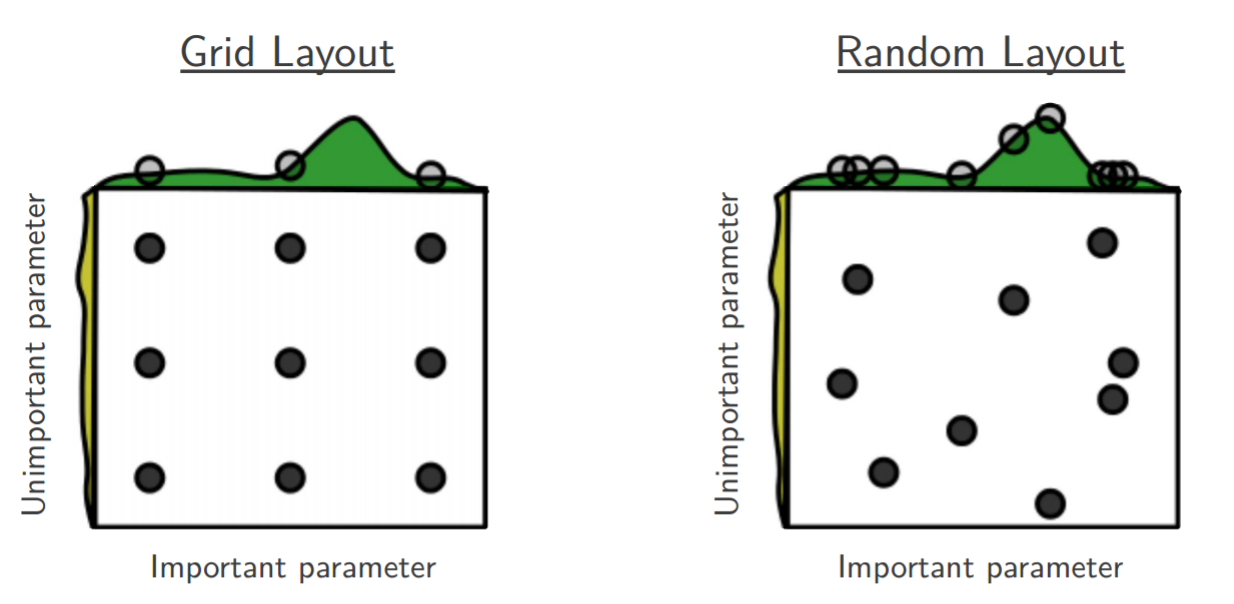
\includegraphics[width=0.99\linewidth]{images/Bergstra12a_hyperparameter_grid_vs_random}
	\caption{A comparison between a grid search and a random search for hyperparameter optimization. In this example, performance is strongly tied to one hyperparameter. The green function represents the effect of an important hyperparameter on a cost function while the yellow function represents the effect for an unimportant hyperparameter. Figure reproduced from [42].}
	\label{fig:Bergstra12a_hyperparameter_grid_vs_random}
\end{figure}


The ability for an ANN to solve a problem depends on the network structure, teaching method, and the training set to be learned. In the following section, a method for generating a training set for isotope identification and quantification is described.

To analyze the performance of a random search, a random hyperparameter efficiency curve, example shown in Figure \ref{fig:Bergstra_random_efficiency_curve_DNN} can be used. In the figure, 256 hyperparameter searches are run. These trials are split into experiments with sizes of increasing powers of two. The best performing trial from each experiment is determined and shown using a box plot.


\begin{figure}[H]
	\centering
	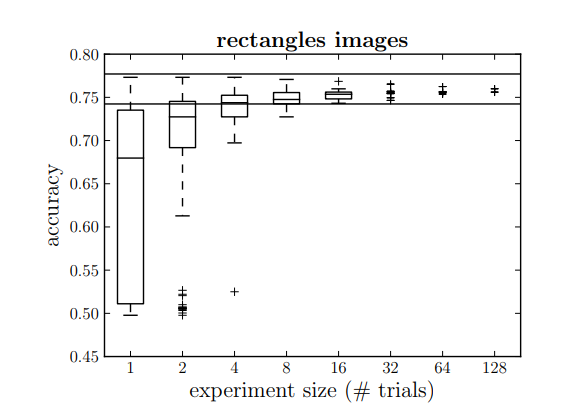
\includegraphics[width=0.9\linewidth]{model_choice_hyperparameter_search_images/Bergstra12_random_efficiency_curve}
	\caption{Example random efficiency curves for a neural network \cite{Bergstra2012}.}
	\label{fig:Bergstra_random_efficiency_curve_DNN}
\end{figure}

\subsection{Additional Machine Learning Models}

In addition to dense models, we also include convolutional and autoencoder models in this work. Convolutional models 

\subsubsection{Convolutional Neural Networks}

Before the popularization of machine learning, many pattern recognition algorithms relied on hand-crafted feature extractors (e.g. manually creating features using edge and line detectors for face recognition) and a simple trainable classifier like a linear model or naive Bayes. There are a number of issues with creating and using custom feature extractors. Robust feature extraction algorithms often require extensive domain knowledge - making them expensive to create. There is rarely a guarantee that these features will be optimal for classification or regression tasks. A classifier created around suboptimal features has the potential to perform poorly in real-world conditions or similar problems.

Deep learning algorithms use a dataset to learn optimum feature extraction and classification techniques simultaneously. CNNs do this by using locally connected convolutional filters instead of fully connected weights. DNNs are fully connected architectures, which means each activation from the previous layer is considered in the next. This leads to redundancy in problems where the input has local structure, like in image recognition or signal processing. Additional CNN layers add hierarchies of representations, meaning that early layers use simple features and deeper layers combine them into more complex features. The magnitude of abstraction can be controlled by tuning the number of convolutional layers in a model. Because low-level features are usually shared among the classes in some data (e.g. edge detection in hand-written digits) the convolutional filters can be shared among classes. This weight sharing decreases the amount of parameters in the model which decreases the probability of overfitting. Weight sharing also makes the model more robust against transformations in the input (e.g. rotations, scaling, and translations).

Figure \ref{fig:cnn_mnist_lecun98} shows one of the first successful CNN architectures, LeNet-5 \cite{Lecun1998}, which classified 32x32 images of handwritten digits using two convolution and average pooling layers followed by two dense layers and an output. This was the first example of a machine learning algorithm creating custom filters and a classification model for the MNIST dataset. 

% AlexNet \cite{Krizhevsky2012} was the first exploration into wider and deeper CNNs. 

% Much more work has been done furthering CNNs. VGG \cite{Simonyan2014} showed that smaller filter sizes are good. 

\begin{figure}[H]
	\centering
	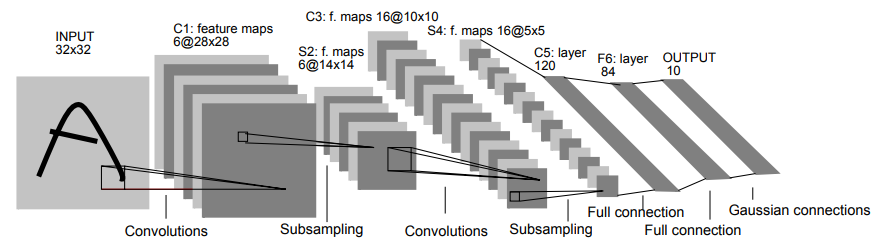
\includegraphics[width=0.85\linewidth]{images/cnn_mnist_lecun98}
	\caption{Architecture of LeNet-5, a CNN created for digit recognition. Image reproduced from \cite{Lecun1998}}
	\label{fig:cnn_mnist_lecun98}
\end{figure}

\subsubsection{Autoencoders} \label{Autoencoders}
% \cite{CHARTE2018} is a practical guide to autoencoders. Great resource.

Autoencoders were introduced by Hinton \cite{Hinton2006} as a generalized nonlinear dimension reduction technique. An autoencoder is a neural network designed to learn a compact representation of some input. This is accomplished by simultaneously training an \textit{encoding network} and a \textit{decoding network}. An example of this can be seen in Figure \ref{fig:Autoencoder_structure}. The encoding ANN reduces an $n-$dimension input signal, $X$, to a $m-$dimension signal, $z$, where $m < n$. The decoding ANN takes the encoded signal, $z$, and reproduces the input signal, $X'$. Once trained, the encoder can pre-train other neural networks or serve as a feature extractor \cite{Erhan2010,CHARTE2018}. 

Methods to encourage the network to learn useful features include forcing the autoencoder to perform denoising \cite{Vincent2008, Vincent2010} and by using an encoding smaller than the input signal (also called an undercomplete autoencoder). Denoising autoencoders corrupt their input with noise, making the autoencoder learn more robust features than those used for simply copying the input. 

% \cite{Masci2011} demonstrated that stacking convolution layers made a good autoencoder.

Other commonly used feature extraction methods are principal component analysis (PCA) \cite{Jolliffe2002}, and linear discriminant analysis (LDA) \cite{Welling2007}. PCA attempts to reduce the dimensionality of a dataset into linearly uncorrelated variables. Using a few of these principle components, the data may be represented in a reduced space that contains most of the information present in the original data. Another linear feature extraction method is LDA. LDA is a supervised feature extraction method that finds linear combinations of features that can be used to separate classes. Non-linear feature extraction methods, such as kernel PCA, also exist. Kernel PCA applies a non-linear transform to the input space and applies PCA to the data in this transformed space. For kernel PCA to perform well, the correct kernel must be chosen for a given problem, which is a non-trivial task.

% While autoencoders were touched on in the uranium enrichment work, they have not been explored thoroughly. There is some evidence that the autoencoder was overtrained to the A special case of denoising autoencoders will be explored for the ANSI dataset. 



% In addition to using fully connected autoencoders, a 1-D convolutional autoencoder will also be explored. A DNN does not assume the input has local spatial structure, while a CNN does. Because gamma-ray spectra have local spatial structure in the form of photopeaks and Compton continua, it may be better to use a CNN over a DNN \cite{CHARTE2018}. To test this, the experiment described above will be repeated using a 1-D convolutional autoencoder.


\begin{figure}[H]
\centering
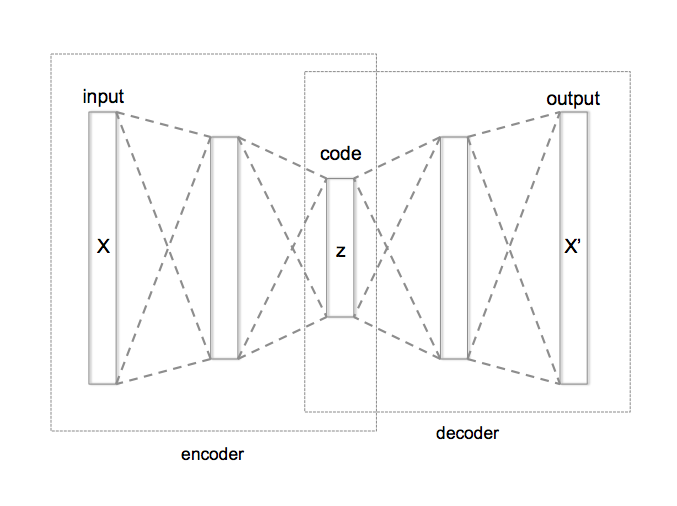
\includegraphics[width=0.8\linewidth]{images/Autoencoder_structure}
\caption{An example of an autoencoder. Image reproduced from \cite{wiki:AutoencoderStructure}.}
\label{fig:Autoencoder_structure}
\end{figure}


% Fully connected ANNs do not assume there is local spatial structure in a signal, so the fully connected ANN would need to learn that there is local structure. Convolutional ANNs assume there is local structure, and the extent of this structure can be changed by changing the length of the convolutional ANNs filters.

% Once the autoencoder is trained, the hidden layer and output layer (representing the reconstructed spectrum) will be used to train a separate ANN for isotope identification and quantification. The performance of these ANNs will be compared.




\section{annsa}

%  \verb|annsa| creates datasets of gamma-ray spectra from spectral templates generated by gamma-ray transport tools.
As a part of this work we developed the open source (under the BSD 3 license) software package \verb|annsa| (Artificial Neural Networks for Spectroscopic Analysis) \cite{annsa}. \verb|annsa| leverages gamma-ray transport software and open source machine learning packages to generate trained machine learning models for spectroscopic tasks. \verb|annsa| contains machine learning models designed for tasks such as: classifying spectra based on an isotope library, quantifying an object's uranium enrichment, and extracting features from a spectrum using autoencoders. Machine learning models included in \verb|annsa| are dense neural networks (DNNs), convolutional neural networks (CNNs), dense autoencoders (DAEs), and convolutional autoencoders (CAEs). We designed \verb|annsa| to be modular, allowing for the addition of extra machine learning models and spectroscopic dataset construction methods. 

% SciPy \cite{scipy},
We also included unit tests using \verb|pytest| \cite{pytest3.5} and the continuous integration framework Circle CI to ensure new functionality can be safely incorporated into \verb|annsa|.

The open source software stack \verb|annsa| uses include: TensorFlow \cite{tensorflow2015-whitepaper} and Keras \cite{chollet2015keras} for the machine learning model creation and training; NumPy \cite{numpy} and pandas \cite{mckinney-proc-scipy-2010} to manipulate and store data; and scikit-learn \cite{scikit-learn} for prepossessing and miscellaneous training tasks. \verb|annsa| can be installed in a UNIX environment using the following commands:
\begin{lstlisting}[language=bash, basicstyle={\small\ttfamily}]
git clone https://github.com/arfc/annsa.git
cd annsa
python setup.py install
\end{lstlisting}
\subsection{Dataset Generation}

The dataset generation process begins by creating a dataset of noiseless template spectra. A gamma-ray transport software and a software that simulates the response from a gamma-ray detector generate the templates. The gamma-ray transport software simulates how photons from each isotope scatter in an environment to reach the detector. Transport software that could be used for this include GADRAS-DRF \cite{mitchell2014}, MCNP \cite{Goorley2016}, or GEANT4 \cite{geant4}. The detector response software accounts for the calibration and Gaussian energy broadening of the detector. \verb|annsa| uses csv formatted template spectra with columns corresponding to simulation settings. An example row from a spectral template csv file in the format used by \verb|annsa| is shown in Figure \ref{fig:template_csv}.

\begin{figure}[H]
	\centering
	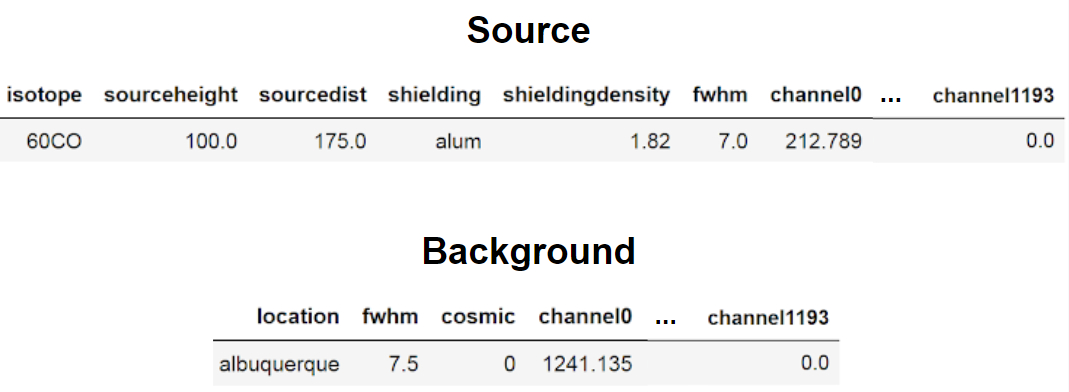
\includegraphics[trim=0 0 0 0,clip,width=1.0\linewidth]{images/template_csv.png}
	\caption{Example spectral template csv entry.}
	\label{fig:template_csv}
\end{figure}

% Datasets are generated using the process outlined in Figure \ref{fig:annsa_data_generation}

A wide variety of realistic gamma-ray spectra can be generated using noiseless templates without the need to excessively run computationally expensive transport software. Spectra with various source-to-background ratios can be simulated by combining source and background templates in desired amounts. This process is displayed in Figure \ref{fig:template_sampling_diagram} for a $^{60}Co$ and background template. First, normalized template spectra generated by the transport software are scaled to the desired total expected counts in the spectrum. In this example, the signal to background ratio is $\frac{1}{5}$ and the expected total number of counts in the final spectrum is 6000. These templates are then added together and sampled using a Poisson distribution to yield spectra with realistic counting statistics. The \verb|annsa| \verb|template_sampling| module contains a function, \verb|make_random_spectrum|, that generates source and background spectra and a function, \verb|make_uenriched_spectrum|, that generates enriched uranium spectra. These functions take a dataset of template spectra and user defined parameters to create new spectra. Using the parameters, these functions choose templates from the template dataset. Chosen templates are combined based on additional parameters such as integration time, calibration, and source-to-background ratio. These spectra and machine learning target values (which isotope is in a spectrum, relative quantities of each isotope in a spectral mixture, $^{235}$U \% enrichment) are stored and saved in a NumPy array for future machine learning training.

\begin{figure}[H]
	\centering
	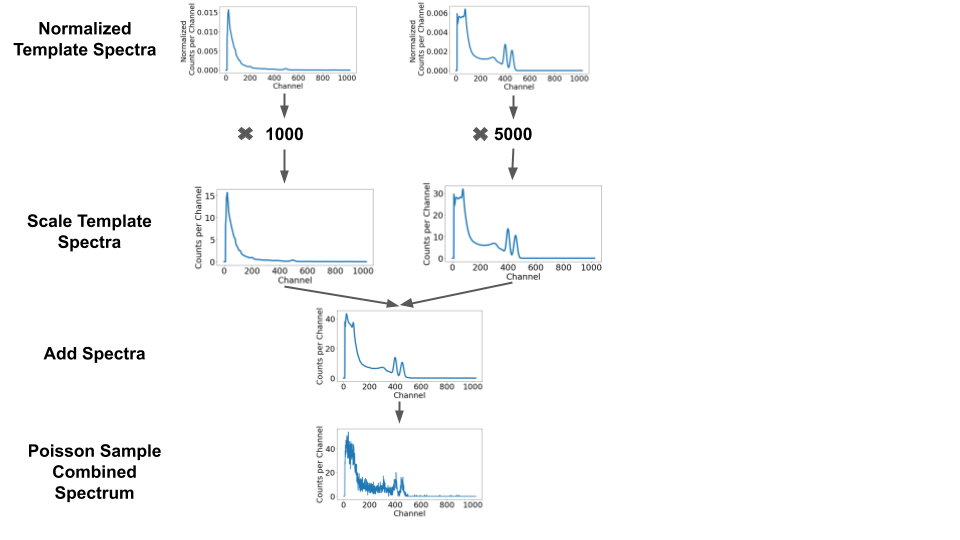
\includegraphics[trim=0 0 350 0,clip,width=1.0\linewidth]{images/template_sampling_diagram.png}
	\caption{An example of the template sampling process combining $^{60}$Co and background template spectra into a dataset entry.}
	\label{fig:template_sampling_diagram}
\end{figure}

This workflow is designed to be flexible and allow for quick dataset prototyping. The workflow can be used for multiple gamma-ray transport and detector response software. Dataset simulation functions can be added or modified in the \verb|template_sampling| module to extend \verb|annsa|'s capabilities.

% trim left bottom right top

% \begin{figure}[H]
% \centering
% 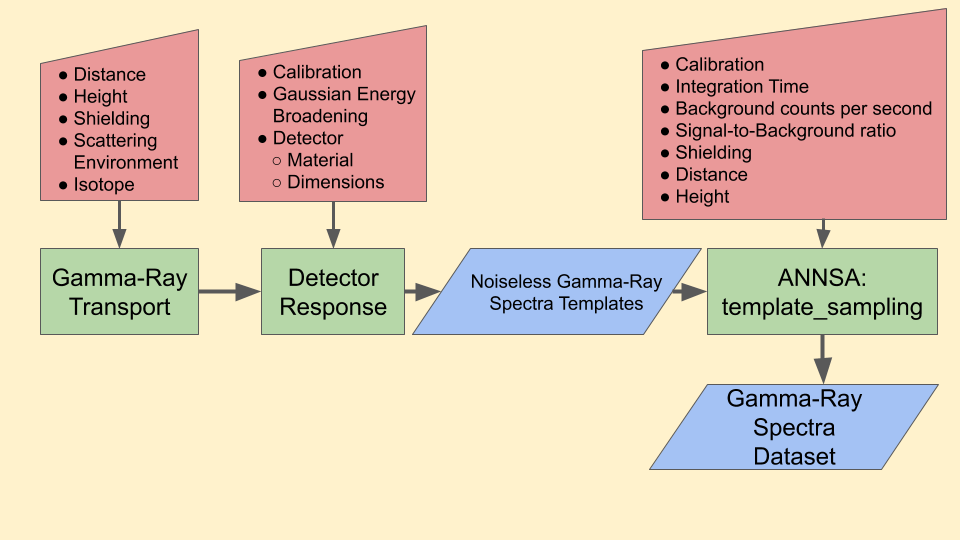
\includegraphics[trim=40 50 10 0,clip,width=0.8\linewidth]{images/annsa_data_generation.png}
% \caption{annsa dataset generation process.}
% \label{fig:annsa_data_generation}
% \end{figure}


\subsection{Machine Learning Models}

\verb|annsa| includes Python functions that build Keras models using the Keras \verb|Sequential| API. The \verb|Sequential| API allows for simple model training and saving. \verb|annsa| includes functions to build DNNs, 1D CNNs, DAEs, and 1D CAEs. This section outlines the architectures available in \verb|annsa|.

% In this way the encoding portion of the autoencoder can be used as a pretrained feature extractor.  Examples of these networks being used are available at \verb|https://github.com/arfc/annsa/examples|.

\subsubsection{Dense Neural Network}

DNNs in \verb|annsa| are created by stacking dense-dropout layers between user defined input and output vectors. An outline of this architecture is shown in Figure \ref{fig:annsa_dnn}. The number of dense-dropout layers and the nodes in each layer are defined by a list of nodes provided by the user. The output length is also user defined, allowing for the training of different sized isotope libraries for classification or training on a single regression target. The input vector length is also defined by the user. Additional necessary user defined parameters are shown in Table \ref{table:annsa_dnn_params}.

\begin{figure}[H]
\centering
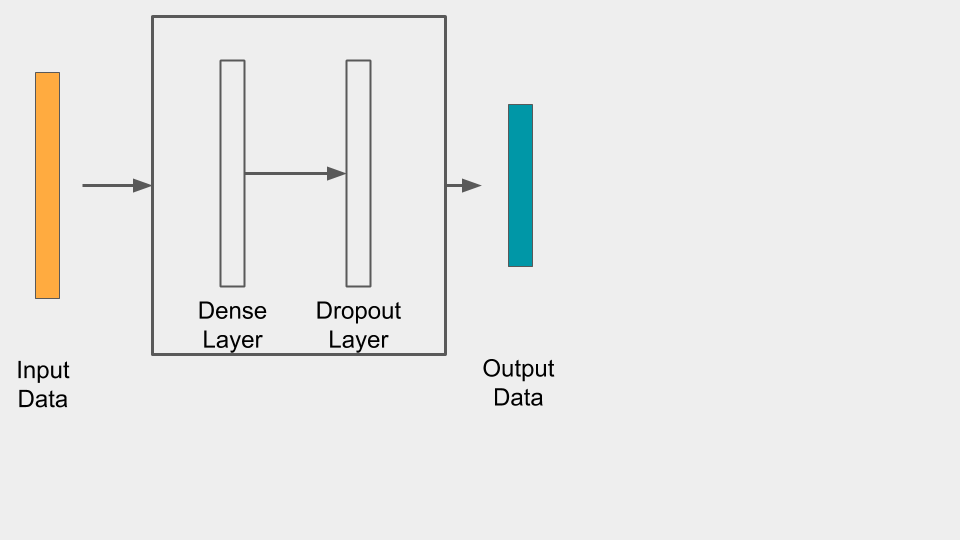
\includegraphics[trim=0 110 380 0,clip,width=0.6\linewidth]{images/annsa_dnn.png}
\caption{ANNSA's DNN structure.}
\label{fig:annsa_dnn}
\end{figure}

\begin{table}[H]
\centering
\caption{ANNSA's DNN parameters.}
\begin{tabular}{c}
\hline
Parameter \\ \hline
Dense Nodes per Layer \\
Dropout Rate \\
Activation Function \\
L2 Regularization Strength \\ 
Minibatch Size \\ 
Input Scaling \\
Output Size \\
Output Activation \\ \hline
\end{tabular}
\label{table:annsa_dnn_params}
\end{table}

\subsubsection{Convolutional Neural Network} \label{annsa_section_conv_neural_network}

The convolution architecture included in \verb|annsa| is based on a 1D convolution followed by a pooling operation. Two 1D convolution-pooling operations are illustrated in Figure \ref{fig:annsa_cnn_fine}. In the convolution, three filters are used. These filters will be referred to as blue, red, and green. Each filter is a vector of the same length, defined by the user. Each filter is convolved along the input and the result is placed in convolutional layer one. This process is illustrated for a single convolution using the red filter. Padding is included at the input signal edges to ensure the resulting convolution has the same length as the input. The pooling operation is indicated by a black box with a white border. Pooling is performed along the output of each filter. In this example max pooling is used with a stride of two. Max pooling takes the maximum value in the pooling length and places it in the next layer. By using a pooling stride of two, the filter is moved by two places before the pooling operation is performed, reducing the output size by a factor of two. Pooling in \verb|annsa| includes zero padding by default to preserve the previous layer's size and to retain information at the signal's ends.

\begin{figure}[H]
	\centering
	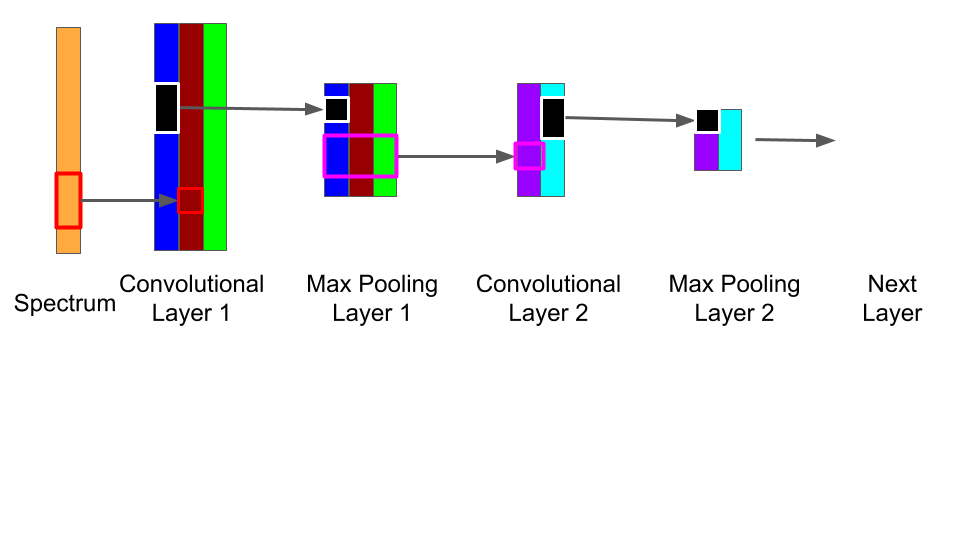
\includegraphics[trim=0 150 40 0,clip,width=0.8\linewidth]{images/annsa_cnn_fine.png}
	\caption{The 1D convolutional-pooling operation included in ANNSA.}
	\label{fig:annsa_cnn_fine}
\end{figure}

Subsequent convolution-pooling layers also use 1D convolutions. In Figure \ref{fig:annsa_cnn_fine}, a second convolution operation is performed using purple and light blue filters. The filters used in each convolutional layer have a depth equal to the number of filters in the previous layer. In the example, this results in the second convolutional layer's filters having a depth of three. Each convolutional layer's filter lengths are mutually independent and defined by the user.


1D CNNs in \verb|annsa| are created by stacking convolutional-pooling layers followed by dense-dropout layers, demonstrated in Figure \ref{fig:annsa_cnn}. The final convolutional layer's output is flattened before being used by the dense layers. Parameters related to the convolutional architecture are shown in Table \ref{table:annsa_cnn_params}. Dropout and L2 regularization are only applied to the dense layers of this network.

\begin{figure}[H]
\centering
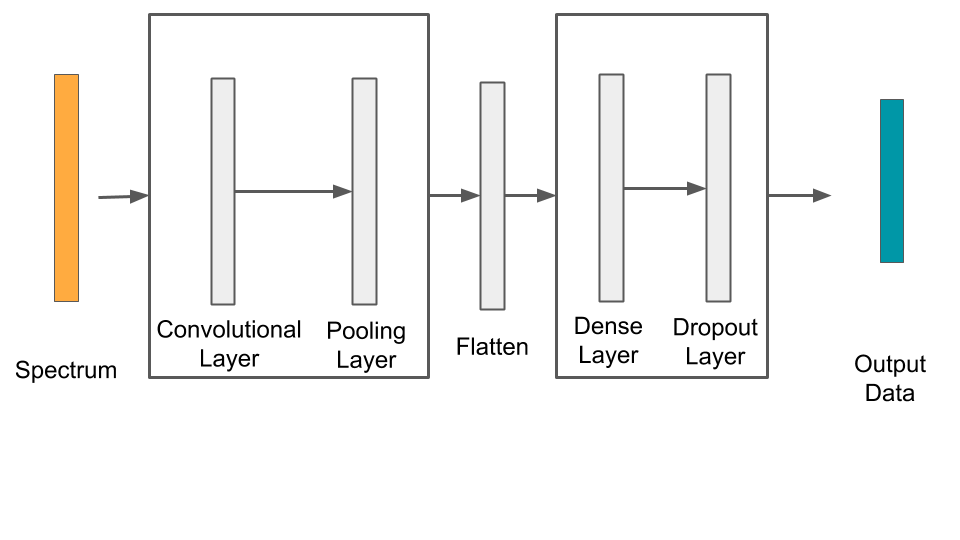
\includegraphics[trim=0 75 20 0,clip,width=0.8\linewidth]{images/annsa_cnn.png}
\caption{ANNSA's CNN structure.}
\label{fig:annsa_cnn}
\end{figure}

\begin{table}[H]
\centering
\caption{ANNSA's 1D CNN parameters.}
\begin{tabular}{c}
\hline
Parameter \\ \hline
Pooling Method \\
Number of Filters per Layer \\
Length of Filter per Layer \\
Convolution Stride per Layer \\
Pooling Stride per Layer \\
Pooling Length per Layer \\
Dense Nodes per Layer \\
Dropout Rate \\
Activation Function \\
L2 Regularization Strength \\ 
Minibatch Size \\ 
Input Scaling \\
Output Size \\
Output Activation \\ \hline
\end{tabular}
\label{table:annsa_cnn_params}
\end{table}

\subsubsection{Dense Autoencoder}

\verb|annsa| includes a class to create DAEs. The DAE class contains an encoder and decoder function. Both functions contain a user defined number of dense-dropout layers and nodes in each layer. Using this, encoders and decoders with different dense architectures can be constructed. Parameters required by the DAE class are shown in Table \ref{table:annsa_dae_params}. An example autoencoder with a two-hidden layer encoder, a single hidden-layer decoder, and no dropout is shown in Figure \ref{fig:annsa_dae}. By changing the input and output, autoencoders can be trained to extract various features from input signals. The final layer of the encoder, called the encoding, contains these extracted features. This example demonstrates a background subtracting denoising autoencoder: the input is a Poisson sampled source and background spectrum and the output is only the source spectrum without Poisson sampling.

\verb|annsa| includes a function in the \verb|load_pretrained_network| module to extract weights from the encoder of a trained DAE and load them into a classification DNN. This process is shown in Figure \ref{fig:annsa_daednn}. This pretrained network can be additionally trained in a process called fine tuning.

\begin{figure}[H]
\centering
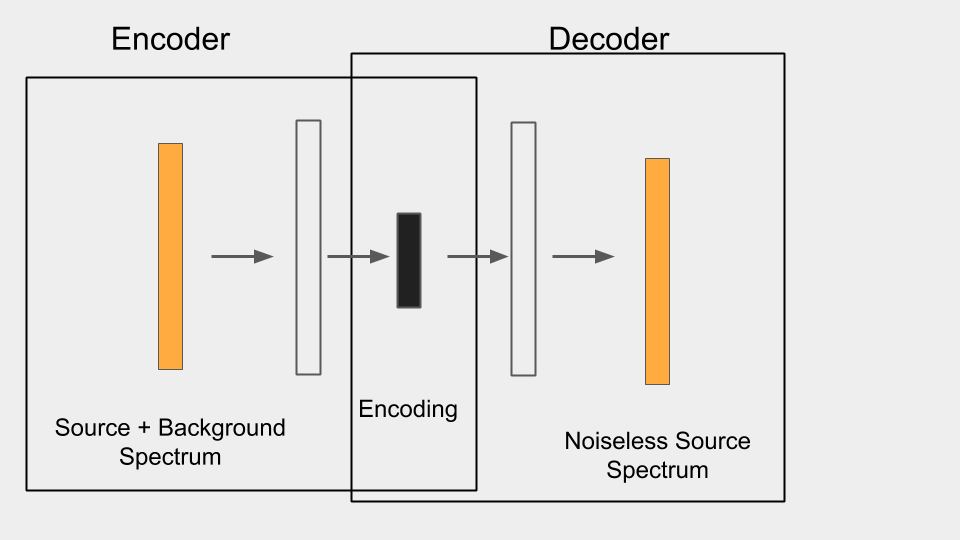
\includegraphics[trim=0 0 125 0,clip,width=0.8\linewidth]{images/annsa_dae.png}
\caption{ANNSA DAE structure. This example demonstrates a background subtracting denoising autoencoder.}
\label{fig:annsa_dae}
\end{figure}

\begin{figure}[H]
\centering
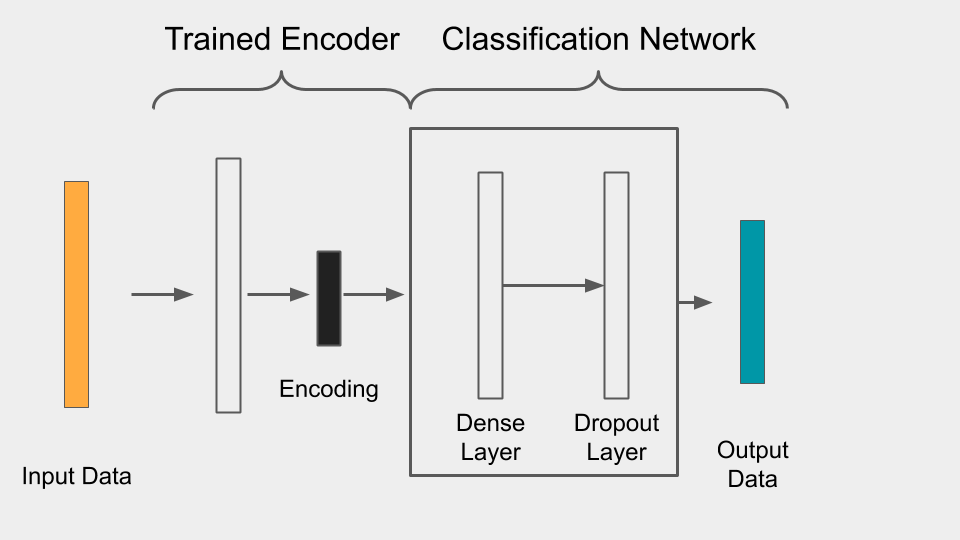
\includegraphics[trim=0 40 85 0,clip,width=0.8\linewidth]{images/annsa_daednn.png}
\caption{An example of a DAE's encoding being loaded into a classification DNN.}
\label{fig:annsa_daednn}
\end{figure}


\begin{table}[H]
\centering
\caption{ANNSA's DAE parameters.}
\begin{tabular}{c}
\hline
Parameter \\ \hline
Dense Encoder Nodes \\
Dense Decoder Nodes \\
Dropout Rate \\
Activation Function \\
Minibatch Size \\ 
Input Scaling \\
Output Size \\
Output Activation \\ \hline
\end{tabular}
\label{table:annsa_dae_params}
\end{table}



\subsubsection{Convolutional Autoencoder}

\verb|annsa| includes a class to create CAEs. Like the DAE, the CAE class contains an encoder and decoder function. The CAE uses parameters from the 1D CNN (Table \ref{fig:annsa_cnn}) with the exception of L2 regularization strength and dropout rate (parameters only used by dense layers). The encoder is constructed using stacked 1D convolutional-pooling layers. As with the CNNs described in section \ref{annsa_section_conv_neural_network}, the CAEs use padding to keep the input and output sizes the same when the strides parameter is set to one. In \verb|annsa| the CAE encoder pooling strides parameter is two by default, making each convolutional-pooling layer reduce the input's length by a factor of two. The decoder uses resize-convolutional layers to increase the dimension of the encoding. The resize layer doubles the input signal's length using bilinear interpolation. The final decoding convolutional layer must have one output filter to ensure the autoencoder's output is a vector. A summary of this operation is shown in Figure \ref{fig:annsa_cae}.

Similar to the DAE, \verb|annsa| includes a function in the \verb|load_pretrained_network| module to extract the weights from the encoder of a trained CAE into a CNN. This process is shown in Figure \ref{fig:annsa_caednn}.

\begin{figure}[H]
\centering
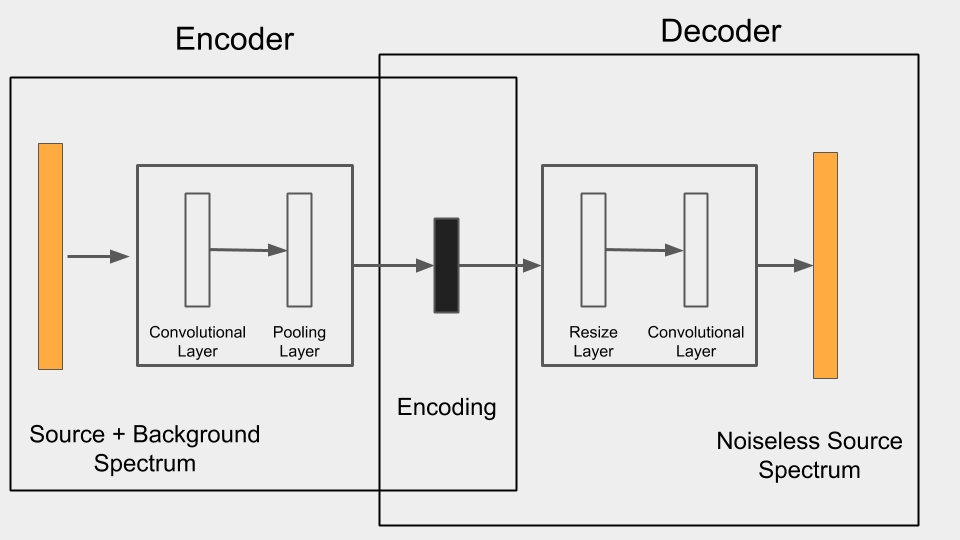
\includegraphics[trim=0 0 30 0,clip,width=1.0\linewidth]{images/annsa_cae.png}
\caption{ANNSA CAE structure. This example demonstrates a background subtracting denoising autoencoder.}
\label{fig:annsa_cae}
\end{figure}

\begin{figure}[H]
\centering
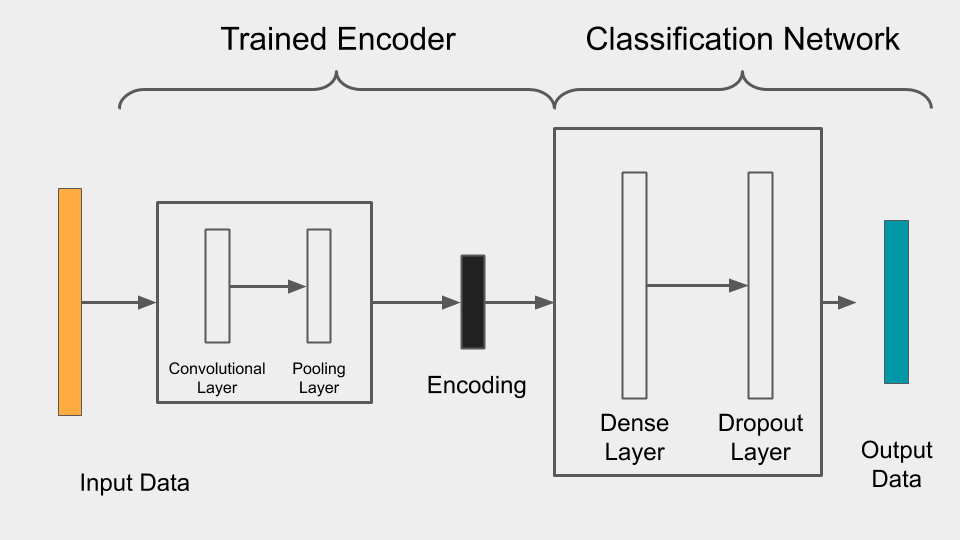
\includegraphics[trim=0 0 0 0,clip,width=0.9\linewidth]{images/annsa_caednn.png}
\caption{An example of a CAE's encoding being loaded into a CNN.}
\label{fig:annsa_caednn}
\end{figure}


\subsection{Training}

Each model was trained using a p2.8xlarge EC2 (Elastic Compute Cloud) instance on Amazon Web Services using the Deep Learning AMI (Amazon Machine Image). Training on multiple GPUs enabled simultaneous training of experiments. Jupyter notebooks used for experiments in this thesis are available at \verb|https://github.com/arfc/annsa/examples|.


\section{Summary}

In this chapter we described the physical processes responsible for signals in gamma-ray spectrometers and how multi-layer ANNs can be trained to solve diverse tasks. We also introduced \verb|annsa|, the Python package we developed and used to create training datasets and train a variety of machine learning models for tasks in gamma-ray spectroscopy. 

In the following chapters, ANNs will be presented using these concepts and their performance on a number of real and simulated spectra will be discussed. 
